\documentclass[11pt]{article}
\usepackage[margin=1in]{geometry}
\usepackage{microtype}
\usepackage{amsmath,amssymb}
\usepackage{booktabs}
\usepackage{graphicx}
\usepackage{xcolor}
\usepackage{caption}
\usepackage{subcaption}
\usepackage[numbers,sort&compress]{natbib}
\usepackage{url}
\usepackage[hidelinks]{hyperref}
\usepackage{fontspec}
\setmainfont{lmroman10-regular.otf}[BoldFont=lmroman10-bold.otf,ItalicFont=lmroman10-italic.otf,BoldItalicFont=lmroman10-bolditalic.otf,SmallCapsFont=lmromancaps10-regular.otf]
\setmonofont{lmmono10-regular.otf}
\newfontfamily\tamilfont{NotoSerifTamil-Regular.ttf}[Path=fonts/,Script=Tamil]   % bundled under the SIL Open Font License (fonts/OFL.txt)
\newcommand{\tamil}[1]{{\tamilfont #1}}
\captionsetup{font=small,labelfont=bf}
\setlength{\bibsep}{3pt}
\setlength{\emergencystretch}{1em}
\newcommand{\nAgreeBpeDanishSd}{0.2}
\newcommand{\nAgreeBpeDanish}{95.7}
\newcommand{\nAgreeBpeEnglishSd}{0.1}
\newcommand{\nAgreeBpeEnglish}{95.2}
\newcommand{\nAgreeBpeSpanishSd}{0.8}
\newcommand{\nAgreeBpeSpanish}{95.1}
\newcommand{\nAgreeBpeTamilSd}{3.4}
\newcommand{\nAgreeBpeTamil}{88.6}
\newcommand{\nAgreeBpeTurkishSd}{1.2}
\newcommand{\nAgreeBpeTurkish}{94.6}
\newcommand{\nAgreeHfBpeDanishSd}{0.1}
\newcommand{\nAgreeHfBpeDanish}{95.9}
\newcommand{\nAgreeHfBpeEnglishSd}{0.1}
\newcommand{\nAgreeHfBpeEnglish}{96.9}
\newcommand{\nAgreeHfBpeSpanishSd}{1.2}
\newcommand{\nAgreeHfBpeSpanish}{95.5}
\newcommand{\nAgreeHfBpeTamilSd}{0.2}
\newcommand{\nAgreeHfBpeTamil}{95.4}
\newcommand{\nAgreeHfBpeTurkishSd}{0.6}
\newcommand{\nAgreeHfBpeTurkish}{95.8}
\newcommand{\nAgreeLtwDanishSd}{0.2}
\newcommand{\nAgreeLtwDanish}{95.8}
\newcommand{\nAgreeLtwEnglishSd}{0.3}
\newcommand{\nAgreeLtwEnglish}{95.2}
\newcommand{\nAgreeLtwSpanishSd}{0.6}
\newcommand{\nAgreeLtwSpanish}{94.9}
\newcommand{\nAgreeLtwTamilSd}{0.2}
\newcommand{\nAgreeLtwTamil}{94.7}
\newcommand{\nAgreeLtwTurkishSd}{0.7}
\newcommand{\nAgreeLtwTurkish}{95.6}
\newcommand{\nAgreePosContentDanishSd}{0.6}
\newcommand{\nAgreePosContentDanish}{95.5}
\newcommand{\nAgreePosContentEnglishSd}{1.1}
\newcommand{\nAgreePosContentEnglish}{95.0}
\newcommand{\nAgreePosContentSpanishSd}{0.1}
\newcommand{\nAgreePosContentSpanish}{95.9}
\newcommand{\nAgreePosContentTamilSd}{0.9}
\newcommand{\nAgreePosContentTamil}{94.0}
\newcommand{\nAgreePosContentTurkishSd}{0.2}
\newcommand{\nAgreePosContentTurkish}{96.0}
\newcommand{\nAgreePosDanishSd}{0.3}
\newcommand{\nAgreePosDanish}{95.5}
\newcommand{\nAgreePosEnglishSd}{0.1}
\newcommand{\nAgreePosEnglish}{95.8}
\newcommand{\nAgreePosPenDanishSd}{0.1}
\newcommand{\nAgreePosPenDanish}{95.5}
\newcommand{\nAgreePosPenEnglishSd}{0.2}
\newcommand{\nAgreePosPenEnglish}{95.6}
\newcommand{\nAgreePosPenSpanishSd}{0.8}
\newcommand{\nAgreePosPenSpanish}{95.1}
\newcommand{\nAgreePosPenTamilSd}{3.5}
\newcommand{\nAgreePosPenTamil}{88.7}
\newcommand{\nAgreePosPenTurkishSd}{1.3}
\newcommand{\nAgreePosPenTurkish}{94.7}
\newcommand{\nAgreePosSpanishSd}{0.9}
\newcommand{\nAgreePosSpanish}{95.2}
\newcommand{\nAgreePosTamilSd}{3.3}
\newcommand{\nAgreePosTamil}{87.5}
\newcommand{\nAgreePosTransDanishSd}{0.3}
\newcommand{\nAgreePosTransDanish}{95.5}
\newcommand{\nAgreePosTransEnglishSd}{0.1}
\newcommand{\nAgreePosTransEnglish}{95.8}
\newcommand{\nAgreePosTransSpanishSd}{0.9}
\newcommand{\nAgreePosTransSpanish}{95.3}
\newcommand{\nAgreePosTransTamilSd}{3.4}
\newcommand{\nAgreePosTransTamil}{87.6}
\newcommand{\nAgreePosTransTurkishSd}{2.7}
\newcommand{\nAgreePosTransTurkish}{92.5}
\newcommand{\nAgreePosTurkishSd}{2.7}
\newcommand{\nAgreePosTurkish}{92.5}
\newcommand{\nAgreeUniDanishSd}{0.2}
\newcommand{\nAgreeUniDanish}{93.5}
\newcommand{\nAgreeUniEnglishSd}{0.1}
\newcommand{\nAgreeUniEnglish}{95.0}
\newcommand{\nAgreeUniSpanishSd}{0.2}
\newcommand{\nAgreeUniSpanish}{94.1}
\newcommand{\nAgreeUniTamilSd}{0.1}
\newcommand{\nAgreeUniTamil}{93.5}
\newcommand{\nAgreeUniTurkishSd}{0.2}
\newcommand{\nAgreeUniTurkish}{94.3}
\newcommand{\nAllPBpeDanish}{22.4}
\newcommand{\nAllPBpeEnglish}{22.1}
\newcommand{\nAllPBpeSpanish}{28.2}
\newcommand{\nAllPBpeTamil}{24.9}
\newcommand{\nAllPBpeTurkish}{25.0}
\newcommand{\nAllPHfBpeDanish}{22.4}
\newcommand{\nAllPHfBpeEnglish}{22.1}
\newcommand{\nAllPHfBpeSpanish}{28.2}
\newcommand{\nAllPHfBpeTamil}{24.9}
\newcommand{\nAllPHfBpeTurkish}{25.0}
\newcommand{\nAllPLtwDanish}{22.4}
\newcommand{\nAllPLtwEnglish}{22.1}
\newcommand{\nAllPLtwSpanish}{28.2}
\newcommand{\nAllPLtwTamil}{24.9}
\newcommand{\nAllPLtwTurkish}{25.0}
\newcommand{\nAllPPosContentDanish}{22.4}
\newcommand{\nAllPPosContentEnglish}{22.1}
\newcommand{\nAllPPosContentSpanish}{28.2}
\newcommand{\nAllPPosContentTamil}{24.9}
\newcommand{\nAllPPosContentTurkish}{25.0}
\newcommand{\nAllPPosDanish}{22.4}
\newcommand{\nAllPPosEnglish}{22.1}
\newcommand{\nAllPPosPenDanish}{22.4}
\newcommand{\nAllPPosPenEnglish}{22.1}
\newcommand{\nAllPPosPenSpanish}{28.2}
\newcommand{\nAllPPosPenTamil}{24.9}
\newcommand{\nAllPPosPenTurkish}{25.0}
\newcommand{\nAllPPosSpanish}{28.2}
\newcommand{\nAllPPosTamil}{24.9}
\newcommand{\nAllPPosTransDanish}{22.4}
\newcommand{\nAllPPosTransEnglish}{22.1}
\newcommand{\nAllPPosTransSpanish}{28.2}
\newcommand{\nAllPPosTransTamil}{24.9}
\newcommand{\nAllPPosTransTurkish}{25.0}
\newcommand{\nAllPPosTurkish}{25.0}
\newcommand{\nAllPUniDanish}{22.4}
\newcommand{\nAllPUniEnglish}{22.1}
\newcommand{\nAllPUniSpanish}{28.2}
\newcommand{\nAllPUniTamil}{24.9}
\newcommand{\nAllPUniTurkish}{25.0}
\newcommand{\nBpcBpeDanishSd}{0.001}
\newcommand{\nBpcBpeDanish}{2.878}
\newcommand{\nBpcBpeEnglishSd}{0.002}
\newcommand{\nBpcBpeEnglish}{2.807}
\newcommand{\nBpcBpeSpanishSd}{0.003}
\newcommand{\nBpcBpeSpanish}{2.689}
\newcommand{\nBpcBpeTamilSd}{0.006}
\newcommand{\nBpcBpeTamil}{2.848}
\newcommand{\nBpcBpeTurkishSd}{0.002}
\newcommand{\nBpcBpeTurkish}{2.963}
\newcommand{\nBpcControlBase}{2.807}
\newcommand{\nBpcControlHigh}{2.805}
\newcommand{\nBpcControlLow}{2.808}
\newcommand{\nBpcHfBpeDanishSd}{0.003}
\newcommand{\nBpcHfBpeDanish}{2.909}
\newcommand{\nBpcHfBpeEnglishSd}{0.003}
\newcommand{\nBpcHfBpeEnglish}{2.715}
\newcommand{\nBpcHfBpeSpanishSd}{0.006}
\newcommand{\nBpcHfBpeSpanish}{2.674}
\newcommand{\nBpcHfBpeTamilSd}{0.001}
\newcommand{\nBpcHfBpeTamil}{2.611}
\newcommand{\nBpcHfBpeTurkishSd}{0.004}
\newcommand{\nBpcHfBpeTurkish}{2.808}
\newcommand{\nBpcLtwDanishSd}{0.001}
\newcommand{\nBpcLtwDanish}{3.007}
\newcommand{\nBpcLtwEnglishSd}{0.003}
\newcommand{\nBpcLtwEnglish}{2.887}
\newcommand{\nBpcLtwSpanishSd}{0.004}
\newcommand{\nBpcLtwSpanish}{2.861}
\newcommand{\nBpcLtwTamilSd}{0.002}
\newcommand{\nBpcLtwTamil}{2.983}
\newcommand{\nBpcLtwTurkishSd}{0.011}
\newcommand{\nBpcLtwTurkish}{3.096}
\newcommand{\nBpcPosContentDanishSd}{0.001}
\newcommand{\nBpcPosContentDanish}{2.868}
\newcommand{\nBpcPosContentEnglishSd}{0.001}
\newcommand{\nBpcPosContentEnglish}{2.794}
\newcommand{\nBpcPosContentSpanishSd}{0.003}
\newcommand{\nBpcPosContentSpanish}{2.680}
\newcommand{\nBpcPosContentTamilSd}{0.015}
\newcommand{\nBpcPosContentTamil}{2.737}
\newcommand{\nBpcPosContentTurkishSd}{0.003}
\newcommand{\nBpcPosContentTurkish}{2.995}
\newcommand{\nBpcPosDanishSd}{0.001}
\newcommand{\nBpcPosDanish}{2.874}
\newcommand{\nBpcPosEnglishSd}{0.001}
\newcommand{\nBpcPosEnglish}{2.785}
\newcommand{\nBpcPosPenDanishSd}{0.001}
\newcommand{\nBpcPosPenDanish}{2.876}
\newcommand{\nBpcPosPenEnglishSd}{0.002}
\newcommand{\nBpcPosPenEnglish}{2.786}
\newcommand{\nBpcPosPenSpanishSd}{0.002}
\newcommand{\nBpcPosPenSpanish}{2.689}
\newcommand{\nBpcPosPenTamilSd}{0.006}
\newcommand{\nBpcPosPenTamil}{2.849}
\newcommand{\nBpcPosPenTurkishSd}{0.003}
\newcommand{\nBpcPosPenTurkish}{2.963}
\newcommand{\nBpcPosSpanishSd}{0.001}
\newcommand{\nBpcPosSpanish}{2.687}
\newcommand{\nBpcPosTamilSd}{0.005}
\newcommand{\nBpcPosTamil}{2.819}
\newcommand{\nBpcPosTransDanishSd}{0.002}
\newcommand{\nBpcPosTransDanish}{2.874}
\newcommand{\nBpcPosTransEnglishSd}{0.001}
\newcommand{\nBpcPosTransEnglish}{2.785}
\newcommand{\nBpcPosTransSpanishSd}{0.001}
\newcommand{\nBpcPosTransSpanish}{2.687}
\newcommand{\nBpcPosTransTamilSd}{0.005}
\newcommand{\nBpcPosTransTamil}{2.819}
\newcommand{\nBpcPosTransTurkishSd}{0.032}
\newcommand{\nBpcPosTransTurkish}{2.935}
\newcommand{\nBpcPosTurkishSd}{0.032}
\newcommand{\nBpcPosTurkish}{2.935}
\newcommand{\nBpcUniDanishSd}{0.007}
\newcommand{\nBpcUniDanish}{2.704}
\newcommand{\nBpcUniEnglishSd}{0.006}
\newcommand{\nBpcUniEnglish}{2.531}
\newcommand{\nBpcUniSpanishSd}{0.011}
\newcommand{\nBpcUniSpanish}{2.473}
\newcommand{\nBpcUniTamilSd}{0.003}
\newcommand{\nBpcUniTamil}{2.524}
\newcommand{\nBpcUniTurkishSd}{0.003}
\newcommand{\nBpcUniTurkish}{2.694}
\newcommand{\nCrossBpeDanishSd}{0.1}
\newcommand{\nCrossBpeDanish}{13.1}
\newcommand{\nCrossBpeEnglishSd}{0.1}
\newcommand{\nCrossBpeEnglish}{15.2}
\newcommand{\nCrossBpeSpanishSd}{0.0}
\newcommand{\nCrossBpeSpanish}{18.3}
\newcommand{\nCrossBpeTamilSd}{1.5}
\newcommand{\nCrossBpeTamil}{22.0}
\newcommand{\nCrossBpeTurkishSd}{0.1}
\newcommand{\nCrossBpeTurkish}{4.5}
\newcommand{\nCrossHfBpeDanishSd}{0.0}
\newcommand{\nCrossHfBpeDanish}{0.0}
\newcommand{\nCrossHfBpeEnglishSd}{0.0}
\newcommand{\nCrossHfBpeEnglish}{0.0}
\newcommand{\nCrossHfBpeSpanishSd}{0.0}
\newcommand{\nCrossHfBpeSpanish}{0.0}
\newcommand{\nCrossHfBpeTamilSd}{0.0}
\newcommand{\nCrossHfBpeTamil}{0.0}
\newcommand{\nCrossHfBpeTurkishSd}{0.0}
\newcommand{\nCrossHfBpeTurkish}{0.0}
\newcommand{\nCrossLtwDanishSd}{0.1}
\newcommand{\nCrossLtwDanish}{15.4}
\newcommand{\nCrossLtwEnglishSd}{0.0}
\newcommand{\nCrossLtwEnglish}{15.7}
\newcommand{\nCrossLtwSpanishSd}{0.0}
\newcommand{\nCrossLtwSpanish}{19.2}
\newcommand{\nCrossLtwTamilSd}{0.2}
\newcommand{\nCrossLtwTamil}{12.8}
\newcommand{\nCrossLtwTurkishSd}{0.1}
\newcommand{\nCrossLtwTurkish}{6.6}
\newcommand{\nCrossPosContentDanishSd}{0.2}
\newcommand{\nCrossPosContentDanish}{9.7}
\newcommand{\nCrossPosContentEnglishSd}{0.2}
\newcommand{\nCrossPosContentEnglish}{10.9}
\newcommand{\nCrossPosContentSpanishSd}{0.1}
\newcommand{\nCrossPosContentSpanish}{14.5}
\newcommand{\nCrossPosContentTamilSd}{0.3}
\newcommand{\nCrossPosContentTamil}{2.2}
\newcommand{\nCrossPosContentTurkishSd}{0.1}
\newcommand{\nCrossPosContentTurkish}{2.5}
\newcommand{\nCrossPosDanishSd}{0.2}
\newcommand{\nCrossPosDanish}{13.2}
\newcommand{\nCrossPosEnglishSd}{0.1}
\newcommand{\nCrossPosEnglish}{14.2}
\newcommand{\nCrossPosPenDanishSd}{0.1}
\newcommand{\nCrossPosPenDanish}{13.2}
\newcommand{\nCrossPosPenEnglishSd}{0.0}
\newcommand{\nCrossPosPenEnglish}{14.4}
\newcommand{\nCrossPosPenSpanishSd}{0.0}
\newcommand{\nCrossPosPenSpanish}{18.3}
\newcommand{\nCrossPosPenTamilSd}{1.5}
\newcommand{\nCrossPosPenTamil}{21.9}
\newcommand{\nCrossPosPenTurkishSd}{0.1}
\newcommand{\nCrossPosPenTurkish}{4.5}
\newcommand{\nCrossPosSpanishSd}{0.0}
\newcommand{\nCrossPosSpanish}{18.4}
\newcommand{\nCrossPosTamilSd}{2.4}
\newcommand{\nCrossPosTamil}{15.6}
\newcommand{\nCrossPosTransDanishSd}{0.2}
\newcommand{\nCrossPosTransDanish}{13.2}
\newcommand{\nCrossPosTransEnglishSd}{0.1}
\newcommand{\nCrossPosTransEnglish}{14.2}
\newcommand{\nCrossPosTransSpanishSd}{0.0}
\newcommand{\nCrossPosTransSpanish}{18.4}
\newcommand{\nCrossPosTransTamilSd}{2.4}
\newcommand{\nCrossPosTransTamil}{15.6}
\newcommand{\nCrossPosTransTurkishSd}{0.1}
\newcommand{\nCrossPosTransTurkish}{4.4}
\newcommand{\nCrossPosTurkishSd}{0.1}
\newcommand{\nCrossPosTurkish}{4.4}
\newcommand{\nCrossUniDanishSd}{0.0}
\newcommand{\nCrossUniDanish}{0.0}
\newcommand{\nCrossUniEnglishSd}{0.0}
\newcommand{\nCrossUniEnglish}{0.0}
\newcommand{\nCrossUniSpanishSd}{0.0}
\newcommand{\nCrossUniSpanish}{0.0}
\newcommand{\nCrossUniTamilSd}{0.0}
\newcommand{\nCrossUniTamil}{0.0}
\newcommand{\nCrossUniTurkishSd}{0.0}
\newcommand{\nCrossUniTurkish}{0.0}
\newcommand{\nFBpeDanishSd}{0.8}
\newcommand{\nFBpeDanish}{24.3}
\newcommand{\nFBpeEnglishSd}{1.6}
\newcommand{\nFBpeEnglish}{40.0}
\newcommand{\nFBpeSpanishSd}{0.8}
\newcommand{\nFBpeSpanish}{18.7}
\newcommand{\nFBpeTamilSd}{2.3}
\newcommand{\nFBpeTamil}{4.4}
\newcommand{\nFBpeTurkishSd}{1.9}
\newcommand{\nFBpeTurkish}{35.0}
\newcommand{\nFHfBpeDanishSd}{0.1}
\newcommand{\nFHfBpeDanish}{13.1}
\newcommand{\nFHfBpeEnglishSd}{0.4}
\newcommand{\nFHfBpeEnglish}{25.5}
\newcommand{\nFHfBpeSpanishSd}{0.5}
\newcommand{\nFHfBpeSpanish}{6.7}
\newcommand{\nFHfBpeTamilSd}{0.3}
\newcommand{\nFHfBpeTamil}{7.5}
\newcommand{\nFHfBpeTurkishSd}{0.4}
\newcommand{\nFHfBpeTurkish}{40.8}
\newcommand{\nFLtwDanishSd}{0.3}
\newcommand{\nFLtwDanish}{43.8}
\newcommand{\nFLtwEnglishSd}{0.1}
\newcommand{\nFLtwEnglish}{59.9}
\newcommand{\nFLtwSpanishSd}{0.1}
\newcommand{\nFLtwSpanish}{36.3}
\newcommand{\nFLtwTamilSd}{0.4}
\newcommand{\nFLtwTamil}{52.9}
\newcommand{\nFLtwTurkishSd}{0.1}
\newcommand{\nFLtwTurkish}{48.7}
\newcommand{\nFPosContentDanishSd}{0.7}
\newcommand{\nFPosContentDanish}{27.8}
\newcommand{\nFPosContentEnglishSd}{0.2}
\newcommand{\nFPosContentEnglish}{43.9}
\newcommand{\nFPosContentSpanishSd}{0.3}
\newcommand{\nFPosContentSpanish}{16.5}
\newcommand{\nFPosContentTamilSd}{1.1}
\newcommand{\nFPosContentTamil}{22.2}
\newcommand{\nFPosContentTurkishSd}{0.4}
\newcommand{\nFPosContentTurkish}{34.2}
\newcommand{\nFPosDanishSd}{0.5}
\newcommand{\nFPosDanish}{24.5}
\newcommand{\nFPosEnglishSd}{1.6}
\newcommand{\nFPosEnglish}{43.4}
\newcommand{\nFPosPenDanishSd}{1.0}
\newcommand{\nFPosPenDanish}{24.4}
\newcommand{\nFPosPenEnglishSd}{1.3}
\newcommand{\nFPosPenEnglish}{42.0}
\newcommand{\nFPosPenSpanishSd}{0.8}
\newcommand{\nFPosPenSpanish}{18.7}
\newcommand{\nFPosPenTamilSd}{2.3}
\newcommand{\nFPosPenTamil}{4.4}
\newcommand{\nFPosPenTurkishSd}{1.9}
\newcommand{\nFPosPenTurkish}{34.9}
\newcommand{\nFPosSpanishSd}{0.8}
\newcommand{\nFPosSpanish}{18.9}
\newcommand{\nFPosTamilSd}{2.3}
\newcommand{\nFPosTamil}{6.2}
\newcommand{\nFPosTransDanishSd}{0.5}
\newcommand{\nFPosTransDanish}{24.5}
\newcommand{\nFPosTransEnglishSd}{1.6}
\newcommand{\nFPosTransEnglish}{43.4}
\newcommand{\nFPosTransSpanishSd}{0.8}
\newcommand{\nFPosTransSpanish}{18.9}
\newcommand{\nFPosTransTamilSd}{2.3}
\newcommand{\nFPosTransTamil}{6.2}
\newcommand{\nFPosTransTurkishSd}{1.6}
\newcommand{\nFPosTransTurkish}{35.1}
\newcommand{\nFPosTurkishSd}{1.6}
\newcommand{\nFPosTurkish}{35.0}
\newcommand{\nFUniDanishSd}{0.5}
\newcommand{\nFUniDanish}{35.1}
\newcommand{\nFUniEnglishSd}{0.5}
\newcommand{\nFUniEnglish}{54.3}
\newcommand{\nFUniSpanishSd}{0.0}
\newcommand{\nFUniSpanish}{29.0}
\newcommand{\nFUniTamilSd}{0.8}
\newcommand{\nFUniTamil}{43.0}
\newcommand{\nFUniTurkishSd}{0.4}
\newcommand{\nFUniTurkish}{46.5}
\newcommand{\nJacBpeDanishSd}{0.4}
\newcommand{\nJacBpeDanish}{76.8}
\newcommand{\nJacBpeEnglishSd}{0.8}
\newcommand{\nJacBpeEnglish}{76.8}
\newcommand{\nJacBpeSpanishSd}{1.8}
\newcommand{\nJacBpeSpanish}{75.8}
\newcommand{\nJacBpeTamilSd}{4.8}
\newcommand{\nJacBpeTamil}{63.8}
\newcommand{\nJacBpeTurkishSd}{1.9}
\newcommand{\nJacBpeTurkish}{74.6}
\newcommand{\nJacHfBpeDanishSd}{0.9}
\newcommand{\nJacHfBpeDanish}{76.1}
\newcommand{\nJacHfBpeEnglishSd}{0.4}
\newcommand{\nJacHfBpeEnglish}{78.5}
\newcommand{\nJacHfBpeSpanishSd}{3.2}
\newcommand{\nJacHfBpeSpanish}{74.4}
\newcommand{\nJacHfBpeTamilSd}{0.2}
\newcommand{\nJacHfBpeTamil}{76.9}
\newcommand{\nJacHfBpeTurkishSd}{1.1}
\newcommand{\nJacHfBpeTurkish}{78.5}
\newcommand{\nJacLtwDanishSd}{0.6}
\newcommand{\nJacLtwDanish}{77.8}
\newcommand{\nJacLtwEnglishSd}{0.7}
\newcommand{\nJacLtwEnglish}{76.9}
\newcommand{\nJacLtwSpanishSd}{1.5}
\newcommand{\nJacLtwSpanish}{75.6}
\newcommand{\nJacLtwTamilSd}{0.5}
\newcommand{\nJacLtwTamil}{74.8}
\newcommand{\nJacLtwTurkishSd}{3.1}
\newcommand{\nJacLtwTurkish}{74.1}
\newcommand{\nJacPosContentDanishSd}{2.4}
\newcommand{\nJacPosContentDanish}{74.3}
\newcommand{\nJacPosContentEnglishSd}{3.1}
\newcommand{\nJacPosContentEnglish}{74.8}
\newcommand{\nJacPosContentSpanishSd}{0.3}
\newcommand{\nJacPosContentSpanish}{77.2}
\newcommand{\nJacPosContentTamilSd}{2.5}
\newcommand{\nJacPosContentTamil}{71.5}
\newcommand{\nJacPosContentTurkishSd}{1.0}
\newcommand{\nJacPosContentTurkish}{77.0}
\newcommand{\nJacPosDanishSd}{0.6}
\newcommand{\nJacPosDanish}{76.7}
\newcommand{\nJacPosEnglishSd}{0.9}
\newcommand{\nJacPosEnglish}{77.8}
\newcommand{\nJacPosPenDanishSd}{0.4}
\newcommand{\nJacPosPenDanish}{76.3}
\newcommand{\nJacPosPenEnglishSd}{0.7}
\newcommand{\nJacPosPenEnglish}{77.1}
\newcommand{\nJacPosPenSpanishSd}{1.8}
\newcommand{\nJacPosPenSpanish}{75.8}
\newcommand{\nJacPosPenTamilSd}{4.8}
\newcommand{\nJacPosPenTamil}{64.1}
\newcommand{\nJacPosPenTurkishSd}{2.3}
\newcommand{\nJacPosPenTurkish}{75.1}
\newcommand{\nJacPosSpanishSd}{2.0}
\newcommand{\nJacPosSpanish}{76.3}
\newcommand{\nJacPosTamilSd}{5.4}
\newcommand{\nJacPosTamil}{61.9}
\newcommand{\nJacPosTransDanishSd}{0.5}
\newcommand{\nJacPosTransDanish}{76.6}
\newcommand{\nJacPosTransEnglishSd}{0.9}
\newcommand{\nJacPosTransEnglish}{77.8}
\newcommand{\nJacPosTransSpanishSd}{2.0}
\newcommand{\nJacPosTransSpanish}{76.2}
\newcommand{\nJacPosTransTamilSd}{5.4}
\newcommand{\nJacPosTransTamil}{61.8}
\newcommand{\nJacPosTransTurkishSd}{7.4}
\newcommand{\nJacPosTransTurkish}{67.2}
\newcommand{\nJacPosTurkishSd}{7.4}
\newcommand{\nJacPosTurkish}{67.1}
\newcommand{\nJacUniDanishSd}{0.2}
\newcommand{\nJacUniDanish}{62.7}
\newcommand{\nJacUniEnglishSd}{1.1}
\newcommand{\nJacUniEnglish}{69.3}
\newcommand{\nJacUniSpanishSd}{0.7}
\newcommand{\nJacUniSpanish}{66.3}
\newcommand{\nJacUniTamilSd}{0.6}
\newcommand{\nJacUniTamil}{62.9}
\newcommand{\nJacUniTurkishSd}{0.4}
\newcommand{\nJacUniTurkish}{69.1}
\newcommand{\nLlmFDanish}{49.0}
\newcommand{\nLlmFEnglish}{83.8}
\newcommand{\nLlmFSpanish}{46.8}
\newcommand{\nLlmFTamil}{80.5}
\newcommand{\nLlmFTurkish}{66.5}
\newcommand{\nLlmInputTokens}{2,048}
\newcommand{\nLlmInvalidDanish}{0}
\newcommand{\nLlmInvalidEnglish}{0}
\newcommand{\nLlmInvalidSpanish}{1}
\newcommand{\nLlmInvalidTamil}{7}
\newcommand{\nLlmInvalidTurkish}{0}
\newcommand{\nLlmNDanish}{400}
\newcommand{\nLlmNEnglish}{400}
\newcommand{\nLlmNSpanish}{399}
\newcommand{\nLlmNTamil}{393}
\newcommand{\nLlmNTurkish}{400}
\newcommand{\nLlmOutputTokens}{4,398}
\newcommand{\nLlmPDanish}{38.9}
\newcommand{\nLlmPEnglish}{77.6}
\newcommand{\nLlmPSpanish}{35.1}
\newcommand{\nLlmPTamil}{72.6}
\newcommand{\nLlmPTurkish}{50.7}
\newcommand{\nLlmRDanish}{66.0}
\newcommand{\nLlmREnglish}{91.0}
\newcommand{\nLlmRSpanish}{69.9}
\newcommand{\nLlmRTamil}{90.4}
\newcommand{\nLlmRTurkish}{96.5}
\newcommand{\nLlmSampleBpeRDanish}{42.0}
\newcommand{\nLlmSampleBpeREnglish}{52.2}
\newcommand{\nLlmSampleBpeRSpanish}{25.3}
\newcommand{\nLlmSampleBpeRTamil}{6.8}
\newcommand{\nLlmSampleBpeRTurkish}{60.2}
\newcommand{\nLlmSampleLtwRDanish}{72.5}
\newcommand{\nLlmSampleLtwREnglish}{87.0}
\newcommand{\nLlmSampleLtwRSpanish}{62.2}
\newcommand{\nLlmSampleLtwRTamil}{84.8}
\newcommand{\nLlmSampleLtwRTurkish}{84.8}
\newcommand{\nLlmSampleUniRDanish}{50.0}
\newcommand{\nLlmSampleUniREnglish}{69.2}
\newcommand{\nLlmSampleUniRSpanish}{44.1}
\newcommand{\nLlmSampleUniRTamil}{48.9}
\newcommand{\nLlmSampleUniRTurkish}{67.2}
\newcommand{\nLlmTpwDanish}{2.69}
\newcommand{\nLlmTpwEnglish}{2.17}
\newcommand{\nLlmTpwSpanish}{2.99}
\newcommand{\nLlmTpwTamil}{2.25}
\newcommand{\nLlmTpwTurkish}{2.90}
\newcommand{\nLtwLexiconAllPDanish}{31.7}
\newcommand{\nLtwLexiconAllPEnglish}{45.3}
\newcommand{\nLtwLexiconAllPSpanish}{25.6}
\newcommand{\nLtwLexiconAllPTamil}{38.5}
\newcommand{\nLtwLexiconAllPTurkish}{34.4}
\newcommand{\nLtwLexiconAllRDanish}{70.8}
\newcommand{\nLtwLexiconAllREnglish}{88.2}
\newcommand{\nLtwLexiconAllRSpanish}{62.2}
\newcommand{\nLtwLexiconAllRTamil}{84.5}
\newcommand{\nLtwLexiconAllRTurkish}{83.3}
\newcommand{\nLtwLexiconTestPDanish}{27.2}
\newcommand{\nLtwLexiconTestPEnglish}{37.2}
\newcommand{\nLtwLexiconTestPSpanish}{18.3}
\newcommand{\nLtwLexiconTestPTamil}{34.7}
\newcommand{\nLtwLexiconTestPTurkish}{32.0}
\newcommand{\nLtwLexiconTestRDanish}{65.5}
\newcommand{\nLtwLexiconTestREnglish}{84.0}
\newcommand{\nLtwLexiconTestRSpanish}{48.1}
\newcommand{\nLtwLexiconTestRTamil}{80.6}
\newcommand{\nLtwLexiconTestRTurkish}{82.7}
\newcommand{\nLtwLexiconUnseenPDanish}{17.9}
\newcommand{\nLtwLexiconUnseenPEnglish}{30.3}
\newcommand{\nLtwLexiconUnseenPSpanish}{15.3}
\newcommand{\nLtwLexiconUnseenPTamil}{27.4}
\newcommand{\nLtwLexiconUnseenPTurkish}{31.2}
\newcommand{\nLtwLexiconUnseenRDanish}{49.5}
\newcommand{\nLtwLexiconUnseenREnglish}{73.7}
\newcommand{\nLtwLexiconUnseenRSpanish}{40.2}
\newcommand{\nLtwLexiconUnseenRTamil}{74.2}
\newcommand{\nLtwLexiconUnseenRTurkish}{81.7}
\newcommand{\nLtwOnlineAllPDanish}{43.6}
\newcommand{\nLtwOnlineAllPEnglish}{50.9}
\newcommand{\nLtwOnlineAllPSpanish}{39.0}
\newcommand{\nLtwOnlineAllPTamil}{46.3}
\newcommand{\nLtwOnlineAllPTurkish}{37.6}
\newcommand{\nLtwOnlineAllRDanish}{97.2}
\newcommand{\nLtwOnlineAllREnglish}{98.2}
\newcommand{\nLtwOnlineAllRSpanish}{99.1}
\newcommand{\nLtwOnlineAllRTamil}{97.6}
\newcommand{\nLtwOnlineAllRTurkish}{88.6}
\newcommand{\nLtwOnlineTestPDanish}{37.0}
\newcommand{\nLtwOnlineTestPEnglish}{40.9}
\newcommand{\nLtwOnlineTestPSpanish}{34.2}
\newcommand{\nLtwOnlineTestPTamil}{39.9}
\newcommand{\nLtwOnlineTestPTurkish}{35.6}
\newcommand{\nLtwOnlineTestRDanish}{88.0}
\newcommand{\nLtwOnlineTestREnglish}{91.1}
\newcommand{\nLtwOnlineTestRSpanish}{94.8}
\newcommand{\nLtwOnlineTestRTamil}{91.5}
\newcommand{\nLtwOnlineTestRTurkish}{89.1}
\newcommand{\nLtwOnlineUnseenPDanish}{35.3}
\newcommand{\nLtwOnlineUnseenPEnglish}{41.1}
\newcommand{\nLtwOnlineUnseenPSpanish}{35.4}
\newcommand{\nLtwOnlineUnseenPTamil}{38.5}
\newcommand{\nLtwOnlineUnseenPTurkish}{34.8}
\newcommand{\nLtwOnlineUnseenRDanish}{97.1}
\newcommand{\nLtwOnlineUnseenREnglish}{98.2}
\newcommand{\nLtwOnlineUnseenRSpanish}{99.1}
\newcommand{\nLtwOnlineUnseenRTamil}{97.7}
\newcommand{\nLtwOnlineUnseenRTurkish}{88.4}
\newcommand{\nMorphTestDanish}{466}
\newcommand{\nMorphTestEnglish}{198}
\newcommand{\nMorphTestSpanish}{347}
\newcommand{\nMorphTestTamil}{180}
\newcommand{\nMorphTestTurkish}{1,940}
\newcommand{\nMorphUnseenDanish}{3,672}
\newcommand{\nMorphUnseenEnglish}{1,685}
\newcommand{\nMorphUnseenSpanish}{4,110}
\newcommand{\nMorphUnseenTamil}{653}
\newcommand{\nMorphUnseenTurkish}{23,891}
\newcommand{\nMorphWordsDanish}{6,650}
\newcommand{\nMorphWordsEnglish}{4,089}
\newcommand{\nMorphWordsSpanish}{6,712}
\newcommand{\nMorphWordsTamil}{1,193}
\newcommand{\nMorphWordsTurkish}{30,192}
\newcommand{\nPBpeDanishSd}{0.6}
\newcommand{\nPBpeDanish}{17.9}
\newcommand{\nPBpeEnglishSd}{1.2}
\newcommand{\nPBpeEnglish}{31.6}
\newcommand{\nPBpeSpanishSd}{0.5}
\newcommand{\nPBpeSpanish}{13.7}
\newcommand{\nPBpeTamilSd}{1.7}
\newcommand{\nPBpeTamil}{3.2}
\newcommand{\nPBpeTurkishSd}{1.4}
\newcommand{\nPBpeTurkish}{24.7}
\newcommand{\nPHfBpeDanishSd}{0.1}
\newcommand{\nPHfBpeDanish}{10.2}
\newcommand{\nPHfBpeEnglishSd}{0.3}
\newcommand{\nPHfBpeEnglish}{22.0}
\newcommand{\nPHfBpeSpanishSd}{0.4}
\newcommand{\nPHfBpeSpanish}{5.3}
\newcommand{\nPHfBpeTamilSd}{0.3}
\newcommand{\nPHfBpeTamil}{6.4}
\newcommand{\nPHfBpeTurkishSd}{0.3}
\newcommand{\nPHfBpeTurkish}{31.0}
\newcommand{\nPLtwDanishSd}{0.2}
\newcommand{\nPLtwDanish}{31.7}
\newcommand{\nPLtwEnglishSd}{0.1}
\newcommand{\nPLtwEnglish}{45.3}
\newcommand{\nPLtwSpanishSd}{0.1}
\newcommand{\nPLtwSpanish}{25.6}
\newcommand{\nPLtwTamilSd}{0.4}
\newcommand{\nPLtwTamil}{38.5}
\newcommand{\nPLtwTurkishSd}{0.1}
\newcommand{\nPLtwTurkish}{34.4}
\newcommand{\nPPosContentDanishSd}{0.5}
\newcommand{\nPPosContentDanish}{20.1}
\newcommand{\nPPosContentEnglishSd}{0.2}
\newcommand{\nPPosContentEnglish}{34.3}
\newcommand{\nPPosContentSpanishSd}{0.2}
\newcommand{\nPPosContentSpanish}{12.1}
\newcommand{\nPPosContentTamilSd}{0.9}
\newcommand{\nPPosContentTamil}{16.8}
\newcommand{\nPPosContentTurkishSd}{0.3}
\newcommand{\nPPosContentTurkish}{24.2}
\newcommand{\nPPosDanishSd}{0.3}
\newcommand{\nPPosDanish}{18.1}
\newcommand{\nPPosEnglishSd}{1.1}
\newcommand{\nPPosEnglish}{33.6}
\newcommand{\nPPosPenDanishSd}{0.7}
\newcommand{\nPPosPenDanish}{18.0}
\newcommand{\nPPosPenEnglishSd}{0.9}
\newcommand{\nPPosPenEnglish}{32.7}
\newcommand{\nPPosPenSpanishSd}{0.5}
\newcommand{\nPPosPenSpanish}{13.7}
\newcommand{\nPPosPenTamilSd}{1.7}
\newcommand{\nPPosPenTamil}{3.2}
\newcommand{\nPPosPenTurkishSd}{1.5}
\newcommand{\nPPosPenTurkish}{24.6}
\newcommand{\nPPosSpanishSd}{0.6}
\newcommand{\nPPosSpanish}{13.8}
\newcommand{\nPPosTamilSd}{1.7}
\newcommand{\nPPosTamil}{4.5}
\newcommand{\nPPosTransDanishSd}{0.3}
\newcommand{\nPPosTransDanish}{18.1}
\newcommand{\nPPosTransEnglishSd}{1.2}
\newcommand{\nPPosTransEnglish}{33.6}
\newcommand{\nPPosTransSpanishSd}{0.6}
\newcommand{\nPPosTransSpanish}{13.8}
\newcommand{\nPPosTransTamilSd}{1.7}
\newcommand{\nPPosTransTamil}{4.6}
\newcommand{\nPPosTransTurkishSd}{1.3}
\newcommand{\nPPosTransTurkish}{24.6}
\newcommand{\nPPosTurkishSd}{1.3}
\newcommand{\nPPosTurkish}{24.6}
\newcommand{\nPUniDanishSd}{0.4}
\newcommand{\nPUniDanish}{27.2}
\newcommand{\nPUniEnglishSd}{0.5}
\newcommand{\nPUniEnglish}{45.0}
\newcommand{\nPUniSpanishSd}{0.0}
\newcommand{\nPUniSpanish}{21.9}
\newcommand{\nPUniTamilSd}{0.8}
\newcommand{\nPUniTamil}{36.9}
\newcommand{\nPUniTurkishSd}{0.3}
\newcommand{\nPUniTurkish}{35.0}
\newcommand{\nRBpeDanishSd}{1.5}
\newcommand{\nRBpeDanish}{37.9}
\newcommand{\nRBpeEnglishSd}{2.6}
\newcommand{\nRBpeEnglish}{54.4}
\newcommand{\nRBpeSpanishSd}{1.5}
\newcommand{\nRBpeSpanish}{29.4}
\newcommand{\nRBpeTamilSd}{3.7}
\newcommand{\nRBpeTamil}{7.4}
\newcommand{\nRBpeTurkishSd}{2.4}
\newcommand{\nRBpeTurkish}{60.2}
\newcommand{\nRHfBpeDanishSd}{0.2}
\newcommand{\nRHfBpeDanish}{18.4}
\newcommand{\nRHfBpeEnglishSd}{0.4}
\newcommand{\nRHfBpeEnglish}{30.3}
\newcommand{\nRHfBpeSpanishSd}{0.7}
\newcommand{\nRHfBpeSpanish}{9.1}
\newcommand{\nRHfBpeTamilSd}{0.4}
\newcommand{\nRHfBpeTamil}{9.0}
\newcommand{\nRHfBpeTurkishSd}{0.7}
\newcommand{\nRHfBpeTurkish}{59.6}
\newcommand{\nRLtwDanishSd}{0.5}
\newcommand{\nRLtwDanish}{70.8}
\newcommand{\nRLtwEnglishSd}{0.1}
\newcommand{\nRLtwEnglish}{88.2}
\newcommand{\nRLtwSpanishSd}{0.3}
\newcommand{\nRLtwSpanish}{62.2}
\newcommand{\nRLtwTamilSd}{0.5}
\newcommand{\nRLtwTamil}{84.5}
\newcommand{\nRLtwTurkishSd}{0.3}
\newcommand{\nRLtwTurkish}{83.3}
\newcommand{\nRPosContentDanishSd}{1.1}
\newcommand{\nRPosContentDanish}{44.8}
\newcommand{\nRPosContentEnglishSd}{0.3}
\newcommand{\nRPosContentEnglish}{60.8}
\newcommand{\nRPosContentSpanishSd}{0.5}
\newcommand{\nRPosContentSpanish}{25.9}
\newcommand{\nRPosContentTamilSd}{1.6}
\newcommand{\nRPosContentTamil}{32.7}
\newcommand{\nRPosContentTurkishSd}{0.4}
\newcommand{\nRPosContentTurkish}{57.8}
\newcommand{\nRPosDanishSd}{1.3}
\newcommand{\nRPosDanish}{37.9}
\newcommand{\nRPosEnglishSd}{2.5}
\newcommand{\nRPosEnglish}{61.3}
\newcommand{\nRPosPenDanishSd}{1.6}
\newcommand{\nRPosPenDanish}{37.9}
\newcommand{\nRPosPenEnglishSd}{2.0}
\newcommand{\nRPosPenEnglish}{58.7}
\newcommand{\nRPosPenSpanishSd}{1.5}
\newcommand{\nRPosPenSpanish}{29.4}
\newcommand{\nRPosPenTamilSd}{3.7}
\newcommand{\nRPosPenTamil}{7.4}
\newcommand{\nRPosPenTurkishSd}{2.5}
\newcommand{\nRPosPenTurkish}{60.1}
\newcommand{\nRPosSpanishSd}{1.5}
\newcommand{\nRPosSpanish}{29.8}
\newcommand{\nRPosTamilSd}{3.3}
\newcommand{\nRPosTamil}{9.5}
\newcommand{\nRPosTransDanishSd}{1.3}
\newcommand{\nRPosTransDanish}{37.9}
\newcommand{\nRPosTransEnglishSd}{2.5}
\newcommand{\nRPosTransEnglish}{61.3}
\newcommand{\nRPosTransSpanishSd}{1.5}
\newcommand{\nRPosTransSpanish}{29.8}
\newcommand{\nRPosTransTamilSd}{3.3}
\newcommand{\nRPosTransTamil}{9.6}
\newcommand{\nRPosTransTurkishSd}{2.1}
\newcommand{\nRPosTransTurkish}{60.7}
\newcommand{\nRPosTurkishSd}{2.1}
\newcommand{\nRPosTurkish}{60.7}
\newcommand{\nRUniDanishSd}{0.6}
\newcommand{\nRUniDanish}{49.3}
\newcommand{\nRUniEnglishSd}{0.4}
\newcommand{\nRUniEnglish}{68.6}
\newcommand{\nRUniSpanishSd}{0.2}
\newcommand{\nRUniSpanish}{42.9}
\newcommand{\nRUniTamilSd}{0.9}
\newcommand{\nRUniTamil}{51.5}
\newcommand{\nRUniTurkishSd}{0.7}
\newcommand{\nRUniTurkish}{69.3}
\newcommand{\nSeeds}{3}
\newcommand{\nSpanPBpeDanish}{21.1}
\newcommand{\nSpanPBpeEnglish}{23.3}
\newcommand{\nSpanPBpeSpanish}{32.3}
\newcommand{\nSpanPBpeTamil}{24.4}
\newcommand{\nSpanPBpeTurkish}{22.3}
\newcommand{\nSpanPHfBpeDanish}{0.0}
\newcommand{\nSpanPHfBpeEnglish}{0.0}
\newcommand{\nSpanPHfBpeSpanish}{0.0}
\newcommand{\nSpanPHfBpeTamil}{0.0}
\newcommand{\nSpanPHfBpeTurkish}{0.0}
\newcommand{\nSpanPLtwDanish}{21.4}
\newcommand{\nSpanPLtwEnglish}{23.0}
\newcommand{\nSpanPLtwSpanish}{31.4}
\newcommand{\nSpanPLtwTamil}{24.4}
\newcommand{\nSpanPLtwTurkish}{22.5}
\newcommand{\nSpanPPosContentDanish}{20.9}
\newcommand{\nSpanPPosContentEnglish}{24.4}
\newcommand{\nSpanPPosContentSpanish}{33.8}
\newcommand{\nSpanPPosContentTamil}{26.5}
\newcommand{\nSpanPPosContentTurkish}{23.7}
\newcommand{\nSpanPPosDanish}{21.1}
\newcommand{\nSpanPPosEnglish}{23.5}
\newcommand{\nSpanPPosPenDanish}{21.1}
\newcommand{\nSpanPPosPenEnglish}{23.5}
\newcommand{\nSpanPPosPenSpanish}{32.3}
\newcommand{\nSpanPPosPenTamil}{24.4}
\newcommand{\nSpanPPosPenTurkish}{22.3}
\newcommand{\nSpanPPosSpanish}{32.3}
\newcommand{\nSpanPPosTamil}{25.0}
\newcommand{\nSpanPPosTransDanish}{21.1}
\newcommand{\nSpanPPosTransEnglish}{23.5}
\newcommand{\nSpanPPosTransSpanish}{32.3}
\newcommand{\nSpanPPosTransTamil}{25.0}
\newcommand{\nSpanPPosTransTurkish}{22.5}
\newcommand{\nSpanPPosTurkish}{22.5}
\newcommand{\nSpanPUniDanish}{0.0}
\newcommand{\nSpanPUniEnglish}{0.0}
\newcommand{\nSpanPUniSpanish}{0.0}
\newcommand{\nSpanPUniTamil}{0.0}
\newcommand{\nSpanPUniTurkish}{0.0}
\newcommand{\nSpanShareBpeDanish}{41.3}
\newcommand{\nSpanShareBpeEnglish}{45.2}
\newcommand{\nSpanShareBpeSpanish}{54.1}
\newcommand{\nSpanShareBpeTamil}{54.1}
\newcommand{\nSpanShareBpeTurkish}{15.5}
\newcommand{\nSpanShareHfBpeDanish}{0.0}
\newcommand{\nSpanShareHfBpeEnglish}{0.0}
\newcommand{\nSpanShareHfBpeSpanish}{0.0}
\newcommand{\nSpanShareHfBpeTamil}{0.0}
\newcommand{\nSpanShareHfBpeTurkish}{0.0}
\newcommand{\nSpanShareLtwDanish}{49.9}
\newcommand{\nSpanShareLtwEnglish}{47.8}
\newcommand{\nSpanShareLtwSpanish}{58.1}
\newcommand{\nSpanShareLtwTamil}{34.2}
\newcommand{\nSpanShareLtwTurkish}{20.9}
\newcommand{\nSpanSharePosContentDanish}{31.0}
\newcommand{\nSpanSharePosContentEnglish}{33.2}
\newcommand{\nSpanSharePosContentSpanish}{43.5}
\newcommand{\nSpanSharePosContentTamil}{7.4}
\newcommand{\nSpanSharePosContentTurkish}{9.0}
\newcommand{\nSpanSharePosDanish}{41.4}
\newcommand{\nSpanSharePosEnglish}{42.6}
\newcommand{\nSpanSharePosPenDanish}{41.3}
\newcommand{\nSpanSharePosPenEnglish}{43.0}
\newcommand{\nSpanSharePosPenSpanish}{54.1}
\newcommand{\nSpanSharePosPenTamil}{54.1}
\newcommand{\nSpanSharePosPenTurkish}{15.6}
\newcommand{\nSpanSharePosSpanish}{54.1}
\newcommand{\nSpanSharePosTamil}{39.5}
\newcommand{\nSpanSharePosTransDanish}{41.4}
\newcommand{\nSpanSharePosTransEnglish}{42.6}
\newcommand{\nSpanSharePosTransSpanish}{54.1}
\newcommand{\nSpanSharePosTransTamil}{39.5}
\newcommand{\nSpanSharePosTransTurkish}{15.2}
\newcommand{\nSpanSharePosTurkish}{15.2}
\newcommand{\nSpanShareUniDanish}{0.0}
\newcommand{\nSpanShareUniEnglish}{0.0}
\newcommand{\nSpanShareUniSpanish}{0.0}
\newcommand{\nSpanShareUniTamil}{0.0}
\newcommand{\nSpanShareUniTurkish}{0.0}
\newcommand{\nSweepFBpeDanishVEightK}{23.3}
\newcommand{\nSweepFBpeDanishVThirtyTwoK}{25.0}
\newcommand{\nSweepFBpeDanishVTwoK}{22.9}
\newcommand{\nSweepFBpeEnglishVEightK}{40.4}
\newcommand{\nSweepFBpeEnglishVThirtyTwoK}{44.1}
\newcommand{\nSweepFBpeEnglishVTwoK}{35.4}
\newcommand{\nSweepFBpeSpanishVEightK}{17.9}
\newcommand{\nSweepFBpeSpanishVThirtyTwoK}{14.8}
\newcommand{\nSweepFBpeSpanishVTwoK}{15.9}
\newcommand{\nSweepFBpeTamilVEightK}{2.9}
\newcommand{\nSweepFBpeTamilVThirtyTwoK}{2.4}
\newcommand{\nSweepFBpeTamilVTwoK}{4.1}
\newcommand{\nSweepFBpeTurkishVEightK}{37.1}
\newcommand{\nSweepFBpeTurkishVThirtyTwoK}{39.2}
\newcommand{\nSweepFBpeTurkishVTwoK}{32.5}
\newcommand{\nSweepFHfBpeDanishVEightK}{13.1}
\newcommand{\nSweepFHfBpeDanishVThirtyTwoK}{10.6}
\newcommand{\nSweepFHfBpeDanishVTwoK}{13.7}
\newcommand{\nSweepFHfBpeEnglishVEightK}{25.6}
\newcommand{\nSweepFHfBpeEnglishVThirtyTwoK}{18.8}
\newcommand{\nSweepFHfBpeEnglishVTwoK}{27.1}
\newcommand{\nSweepFHfBpeSpanishVEightK}{7.2}
\newcommand{\nSweepFHfBpeSpanishVThirtyTwoK}{7.2}
\newcommand{\nSweepFHfBpeSpanishVTwoK}{9.5}
\newcommand{\nSweepFHfBpeTamilVEightK}{7.7}
\newcommand{\nSweepFHfBpeTamilVThirtyTwoK}{6.3}
\newcommand{\nSweepFHfBpeTamilVTwoK}{8.6}
\newcommand{\nSweepFHfBpeTurkishVEightK}{40.4}
\newcommand{\nSweepFHfBpeTurkishVThirtyTwoK}{41.0}
\newcommand{\nSweepFHfBpeTurkishVTwoK}{35.4}
\newcommand{\nSweepFLtwDanishVEightK}{43.5}
\newcommand{\nSweepFLtwDanishVThirtyTwoK}{48.6}
\newcommand{\nSweepFLtwDanishVTwoK}{35.1}
\newcommand{\nSweepFLtwEnglishVEightK}{59.9}
\newcommand{\nSweepFLtwEnglishVThirtyTwoK}{68.1}
\newcommand{\nSweepFLtwEnglishVTwoK}{48.9}
\newcommand{\nSweepFLtwSpanishVEightK}{36.4}
\newcommand{\nSweepFLtwSpanishVThirtyTwoK}{42.8}
\newcommand{\nSweepFLtwSpanishVTwoK}{29.8}
\newcommand{\nSweepFLtwTamilVEightK}{52.8}
\newcommand{\nSweepFLtwTamilVThirtyTwoK}{59.1}
\newcommand{\nSweepFLtwTamilVTwoK}{44.0}
\newcommand{\nSweepFLtwTurkishVEightK}{48.8}
\newcommand{\nSweepFLtwTurkishVThirtyTwoK}{52.9}
\newcommand{\nSweepFLtwTurkishVTwoK}{42.3}
\newcommand{\nSweepFPosContentDanishVEightK}{27.6}
\newcommand{\nSweepFPosContentDanishVThirtyTwoK}{29.3}
\newcommand{\nSweepFPosContentDanishVTwoK}{24.4}
\newcommand{\nSweepFPosContentEnglishVEightK}{43.8}
\newcommand{\nSweepFPosContentEnglishVThirtyTwoK}{49.1}
\newcommand{\nSweepFPosContentEnglishVTwoK}{36.7}
\newcommand{\nSweepFPosContentSpanishVEightK}{16.8}
\newcommand{\nSweepFPosContentSpanishVThirtyTwoK}{17.4}
\newcommand{\nSweepFPosContentSpanishVTwoK}{16.2}
\newcommand{\nSweepFPosContentTamilVEightK}{22.8}
\newcommand{\nSweepFPosContentTamilVThirtyTwoK}{23.2}
\newcommand{\nSweepFPosContentTamilVTwoK}{21.8}
\newcommand{\nSweepFPosContentTurkishVEightK}{33.7}
\newcommand{\nSweepFPosContentTurkishVThirtyTwoK}{35.7}
\newcommand{\nSweepFPosContentTurkishVTwoK}{30.1}
\newcommand{\nSweepFPosDanishVEightK}{23.8}
\newcommand{\nSweepFPosDanishVThirtyTwoK}{25.3}
\newcommand{\nSweepFPosDanishVTwoK}{23.0}
\newcommand{\nSweepFPosEnglishVEightK}{43.7}
\newcommand{\nSweepFPosEnglishVThirtyTwoK}{46.9}
\newcommand{\nSweepFPosEnglishVTwoK}{37.7}
\newcommand{\nSweepFPosPenDanishVEightK}{23.2}
\newcommand{\nSweepFPosPenEnglishVEightK}{42.4}
\newcommand{\nSweepFPosPenSpanishVEightK}{17.9}
\newcommand{\nSweepFPosPenTamilVEightK}{2.9}
\newcommand{\nSweepFPosPenTurkishVEightK}{37.1}
\newcommand{\nSweepFPosSpanishVEightK}{17.9}
\newcommand{\nSweepFPosSpanishVThirtyTwoK}{15.9}
\newcommand{\nSweepFPosSpanishVTwoK}{15.9}
\newcommand{\nSweepFPosTamilVEightK}{5.2}
\newcommand{\nSweepFPosTamilVThirtyTwoK}{4.0}
\newcommand{\nSweepFPosTamilVTwoK}{5.7}
\newcommand{\nSweepFPosTransDanishVEightK}{23.8}
\newcommand{\nSweepFPosTransEnglishVEightK}{43.7}
\newcommand{\nSweepFPosTransSpanishVEightK}{17.9}
\newcommand{\nSweepFPosTransTamilVEightK}{5.3}
\newcommand{\nSweepFPosTransTurkishVEightK}{36.9}
\newcommand{\nSweepFPosTurkishVEightK}{36.9}
\newcommand{\nSweepFPosTurkishVThirtyTwoK}{39.2}
\newcommand{\nSweepFPosTurkishVTwoK}{32.9}
\newcommand{\nSweepFUniDanishVEightK}{35.3}
\newcommand{\nSweepFUniDanishVThirtyTwoK}{29.1}
\newcommand{\nSweepFUniDanishVTwoK}{27.2}
\newcommand{\nSweepFUniEnglishVEightK}{54.4}
\newcommand{\nSweepFUniEnglishVThirtyTwoK}{40.3}
\newcommand{\nSweepFUniEnglishVTwoK}{43.7}
\newcommand{\nSweepFUniSpanishVEightK}{29.0}
\newcommand{\nSweepFUniSpanishVThirtyTwoK}{29.5}
\newcommand{\nSweepFUniSpanishVTwoK}{19.4}
\newcommand{\nSweepFUniTamilVEightK}{42.0}
\newcommand{\nSweepFUniTamilVThirtyTwoK}{29.3}
\newcommand{\nSweepFUniTamilVTwoK}{43.1}
\newcommand{\nSweepFUniTurkishVEightK}{46.3}
\newcommand{\nSweepFUniTurkishVThirtyTwoK}{43.0}
\newcommand{\nSweepFUniTurkishVTwoK}{43.3}
\newcommand{\nSweepTpwBpeDanishVEightK}{1.61}
\newcommand{\nSweepTpwBpeDanishVThirtyTwoK}{1.30}
\newcommand{\nSweepTpwBpeDanishVTwoK}{2.17}
\newcommand{\nSweepTpwBpeEnglishVEightK}{1.48}
\newcommand{\nSweepTpwBpeEnglishVThirtyTwoK}{1.18}
\newcommand{\nSweepTpwBpeEnglishVTwoK}{2.05}
\newcommand{\nSweepTpwBpeSpanishVEightK}{1.41}
\newcommand{\nSweepTpwBpeSpanishVThirtyTwoK}{1.13}
\newcommand{\nSweepTpwBpeSpanishVTwoK}{1.95}
\newcommand{\nSweepTpwBpeTamilVEightK}{2.24}
\newcommand{\nSweepTpwBpeTamilVThirtyTwoK}{1.85}
\newcommand{\nSweepTpwBpeTamilVTwoK}{3.00}
\newcommand{\nSweepTpwBpeTurkishVEightK}{1.96}
\newcommand{\nSweepTpwBpeTurkishVThirtyTwoK}{1.55}
\newcommand{\nSweepTpwBpeTurkishVTwoK}{2.74}
\newcommand{\nSweepTpwHfBpeDanishVEightK}{1.71}
\newcommand{\nSweepTpwHfBpeDanishVThirtyTwoK}{1.42}
\newcommand{\nSweepTpwHfBpeDanishVTwoK}{2.25}
\newcommand{\nSweepTpwHfBpeEnglishVEightK}{1.55}
\newcommand{\nSweepTpwHfBpeEnglishVThirtyTwoK}{1.29}
\newcommand{\nSweepTpwHfBpeEnglishVTwoK}{2.07}
\newcommand{\nSweepTpwHfBpeSpanishVEightK}{1.57}
\newcommand{\nSweepTpwHfBpeSpanishVThirtyTwoK}{1.30}
\newcommand{\nSweepTpwHfBpeSpanishVTwoK}{2.07}
\newcommand{\nSweepTpwHfBpeTamilVEightK}{2.04}
\newcommand{\nSweepTpwHfBpeTamilVThirtyTwoK}{1.64}
\newcommand{\nSweepTpwHfBpeTamilVTwoK}{2.83}
\newcommand{\nSweepTpwHfBpeTurkishVEightK}{1.88}
\newcommand{\nSweepTpwHfBpeTurkishVThirtyTwoK}{1.50}
\newcommand{\nSweepTpwHfBpeTurkishVTwoK}{2.66}
\newcommand{\nSweepTpwLtwDanishVEightK}{1.70}
\newcommand{\nSweepTpwLtwDanishVThirtyTwoK}{1.41}
\newcommand{\nSweepTpwLtwDanishVTwoK}{2.26}
\newcommand{\nSweepTpwLtwEnglishVEightK}{1.54}
\newcommand{\nSweepTpwLtwEnglishVThirtyTwoK}{1.24}
\newcommand{\nSweepTpwLtwEnglishVTwoK}{2.10}
\newcommand{\nSweepTpwLtwSpanishVEightK}{1.53}
\newcommand{\nSweepTpwLtwSpanishVThirtyTwoK}{1.24}
\newcommand{\nSweepTpwLtwSpanishVTwoK}{2.07}
\newcommand{\nSweepTpwLtwTamilVEightK}{2.38}
\newcommand{\nSweepTpwLtwTamilVThirtyTwoK}{1.97}
\newcommand{\nSweepTpwLtwTamilVTwoK}{3.14}
\newcommand{\nSweepTpwLtwTurkishVEightK}{2.07}
\newcommand{\nSweepTpwLtwTurkishVThirtyTwoK}{1.70}
\newcommand{\nSweepTpwLtwTurkishVTwoK}{2.82}
\newcommand{\nSweepTpwPosContentDanishVEightK}{1.62}
\newcommand{\nSweepTpwPosContentDanishVThirtyTwoK}{1.30}
\newcommand{\nSweepTpwPosContentDanishVTwoK}{2.19}
\newcommand{\nSweepTpwPosContentEnglishVEightK}{1.49}
\newcommand{\nSweepTpwPosContentEnglishVThirtyTwoK}{1.17}
\newcommand{\nSweepTpwPosContentEnglishVTwoK}{2.06}
\newcommand{\nSweepTpwPosContentSpanishVEightK}{1.42}
\newcommand{\nSweepTpwPosContentSpanishVThirtyTwoK}{1.13}
\newcommand{\nSweepTpwPosContentSpanishVTwoK}{1.97}
\newcommand{\nSweepTpwPosContentTamilVEightK}{2.14}
\newcommand{\nSweepTpwPosContentTamilVThirtyTwoK}{1.69}
\newcommand{\nSweepTpwPosContentTamilVTwoK}{2.95}
\newcommand{\nSweepTpwPosContentTurkishVEightK}{2.00}
\newcommand{\nSweepTpwPosContentTurkishVThirtyTwoK}{1.58}
\newcommand{\nSweepTpwPosContentTurkishVTwoK}{2.77}
\newcommand{\nSweepTpwPosDanishVEightK}{1.60}
\newcommand{\nSweepTpwPosDanishVThirtyTwoK}{1.30}
\newcommand{\nSweepTpwPosDanishVTwoK}{2.17}
\newcommand{\nSweepTpwPosEnglishVEightK}{1.47}
\newcommand{\nSweepTpwPosEnglishVThirtyTwoK}{1.17}
\newcommand{\nSweepTpwPosEnglishVTwoK}{2.04}
\newcommand{\nSweepTpwPosPenDanishVEightK}{1.61}
\newcommand{\nSweepTpwPosPenEnglishVEightK}{1.47}
\newcommand{\nSweepTpwPosPenSpanishVEightK}{1.41}
\newcommand{\nSweepTpwPosPenTamilVEightK}{2.24}
\newcommand{\nSweepTpwPosPenTurkishVEightK}{1.96}
\newcommand{\nSweepTpwPosSpanishVEightK}{1.41}
\newcommand{\nSweepTpwPosSpanishVThirtyTwoK}{1.13}
\newcommand{\nSweepTpwPosSpanishVTwoK}{1.95}
\newcommand{\nSweepTpwPosTamilVEightK}{2.22}
\newcommand{\nSweepTpwPosTamilVThirtyTwoK}{1.81}
\newcommand{\nSweepTpwPosTamilVTwoK}{2.99}
\newcommand{\nSweepTpwPosTransDanishVEightK}{1.61}
\newcommand{\nSweepTpwPosTransEnglishVEightK}{1.47}
\newcommand{\nSweepTpwPosTransSpanishVEightK}{1.41}
\newcommand{\nSweepTpwPosTransTamilVEightK}{2.22}
\newcommand{\nSweepTpwPosTransTurkishVEightK}{1.91}
\newcommand{\nSweepTpwPosTurkishVEightK}{1.91}
\newcommand{\nSweepTpwPosTurkishVThirtyTwoK}{1.50}
\newcommand{\nSweepTpwPosTurkishVTwoK}{2.70}
\newcommand{\nSweepTpwUniDanishVEightK}{1.78}
\newcommand{\nSweepTpwUniDanishVThirtyTwoK}{1.46}
\newcommand{\nSweepTpwUniDanishVTwoK}{2.30}
\newcommand{\nSweepTpwUniEnglishVEightK}{1.61}
\newcommand{\nSweepTpwUniEnglishVThirtyTwoK}{1.35}
\newcommand{\nSweepTpwUniEnglishVTwoK}{2.12}
\newcommand{\nSweepTpwUniSpanishVEightK}{1.61}
\newcommand{\nSweepTpwUniSpanishVThirtyTwoK}{1.33}
\newcommand{\nSweepTpwUniSpanishVTwoK}{2.08}
\newcommand{\nSweepTpwUniTamilVEightK}{2.18}
\newcommand{\nSweepTpwUniTamilVThirtyTwoK}{1.78}
\newcommand{\nSweepTpwUniTamilVTwoK}{2.86}
\newcommand{\nSweepTpwUniTurkishVEightK}{2.00}
\newcommand{\nSweepTpwUniTurkishVThirtyTwoK}{1.65}
\newcommand{\nSweepTpwUniTurkishVTwoK}{2.69}
\newcommand{\nTestWordsDanish}{34,330}
\newcommand{\nTestWordsEnglish}{40,851}
\newcommand{\nTestWordsSpanish}{42,776}
\newcommand{\nTestWordsTamil}{23,337}
\newcommand{\nTestWordsTurkish}{31,955}
\newcommand{\nTpwBpeDanishSd}{0.002}
\newcommand{\nTpwBpeDanish}{1.606}
\newcommand{\nTpwBpeEnglishSd}{0.002}
\newcommand{\nTpwBpeEnglish}{1.481}
\newcommand{\nTpwBpeSpanishSd}{0.002}
\newcommand{\nTpwBpeSpanish}{1.413}
\newcommand{\nTpwBpeTamilSd}{0.005}
\newcommand{\nTpwBpeTamil}{2.242}
\newcommand{\nTpwBpeTurkishSd}{0.002}
\newcommand{\nTpwBpeTurkish}{1.962}
\newcommand{\nTpwHfBpeDanishSd}{0.001}
\newcommand{\nTpwHfBpeDanish}{1.713}
\newcommand{\nTpwHfBpeEnglishSd}{0.001}
\newcommand{\nTpwHfBpeEnglish}{1.555}
\newcommand{\nTpwHfBpeSpanishSd}{0.000}
\newcommand{\nTpwHfBpeSpanish}{1.565}
\newcommand{\nTpwHfBpeTamilSd}{0.001}
\newcommand{\nTpwHfBpeTamil}{2.042}
\newcommand{\nTpwHfBpeTurkishSd}{0.002}
\newcommand{\nTpwHfBpeTurkish}{1.883}
\newcommand{\nTpwLtwDanishSd}{0.001}
\newcommand{\nTpwLtwDanish}{1.703}
\newcommand{\nTpwLtwEnglishSd}{0.001}
\newcommand{\nTpwLtwEnglish}{1.538}
\newcommand{\nTpwLtwSpanishSd}{0.002}
\newcommand{\nTpwLtwSpanish}{1.531}
\newcommand{\nTpwLtwTamilSd}{0.002}
\newcommand{\nTpwLtwTamil}{2.376}
\newcommand{\nTpwLtwTurkishSd}{0.010}
\newcommand{\nTpwLtwTurkish}{2.080}
\newcommand{\nTpwPosContentDanishSd}{0.001}
\newcommand{\nTpwPosContentDanish}{1.619}
\newcommand{\nTpwPosContentEnglishSd}{0.002}
\newcommand{\nTpwPosContentEnglish}{1.486}
\newcommand{\nTpwPosContentSpanishSd}{0.002}
\newcommand{\nTpwPosContentSpanish}{1.423}
\newcommand{\nTpwPosContentTamilSd}{0.012}
\newcommand{\nTpwPosContentTamil}{2.150}
\newcommand{\nTpwPosContentTurkishSd}{0.003}
\newcommand{\nTpwPosContentTurkish}{1.998}
\newcommand{\nTpwPosDanishSd}{0.002}
\newcommand{\nTpwPosDanish}{1.604}
\newcommand{\nTpwPosEnglishSd}{0.001}
\newcommand{\nTpwPosEnglish}{1.470}
\newcommand{\nTpwPosPenDanishSd}{0.002}
\newcommand{\nTpwPosPenDanish}{1.605}
\newcommand{\nTpwPosPenEnglishSd}{0.001}
\newcommand{\nTpwPosPenEnglish}{1.470}
\newcommand{\nTpwPosPenSpanishSd}{0.002}
\newcommand{\nTpwPosPenSpanish}{1.413}
\newcommand{\nTpwPosPenTamilSd}{0.005}
\newcommand{\nTpwPosPenTamil}{2.243}
\newcommand{\nTpwPosPenTurkishSd}{0.003}
\newcommand{\nTpwPosPenTurkish}{1.962}
\newcommand{\nTpwPosSpanishSd}{0.001}
\newcommand{\nTpwPosSpanish}{1.412}
\newcommand{\nTpwPosTamilSd}{0.006}
\newcommand{\nTpwPosTamil}{2.215}
\newcommand{\nTpwPosTransDanishSd}{0.002}
\newcommand{\nTpwPosTransDanish}{1.604}
\newcommand{\nTpwPosTransEnglishSd}{0.001}
\newcommand{\nTpwPosTransEnglish}{1.470}
\newcommand{\nTpwPosTransSpanishSd}{0.001}
\newcommand{\nTpwPosTransSpanish}{1.412}
\newcommand{\nTpwPosTransTamilSd}{0.006}
\newcommand{\nTpwPosTransTamil}{2.215}
\newcommand{\nTpwPosTransTurkishSd}{0.025}
\newcommand{\nTpwPosTransTurkish}{1.938}
\newcommand{\nTpwPosTurkishSd}{0.025}
\newcommand{\nTpwPosTurkish}{1.938}
\newcommand{\nTpwUniDanishSd}{0.004}
\newcommand{\nTpwUniDanish}{1.778}
\newcommand{\nTpwUniEnglishSd}{0.001}
\newcommand{\nTpwUniEnglish}{1.609}
\newcommand{\nTpwUniSpanishSd}{0.002}
\newcommand{\nTpwUniSpanish}{1.607}
\newcommand{\nTpwUniTamilSd}{0.006}
\newcommand{\nTpwUniTamil}{2.177}
\newcommand{\nTpwUniTurkishSd}{0.004}
\newcommand{\nTpwUniTurkish}{2.004}
\newcommand{\nTrainWordsDanish}{213,460}
\newcommand{\nTrainWordsEnglish}{246,661}
\newcommand{\nTrainWordsSpanish}{249,802}
\newcommand{\nTrainWordsTamil}{143,704}
\newcommand{\nTrainWordsTurkish}{193,551}
\newcommand{\nVocabBudget}{8,000}


\title{Lemma Boundaries Improve Morphological Alignment of Subword Tokenizers but Worsen Language-Model Loss}
\author{%
  Jessie Dong\thanks{Equal contribution.}\\
  Stanford University\\
  \texttt{jessiedong@stanford.edu}
  \and
  Anish Chaudhuri\footnotemark[1]\\
  Stanford University\\
  \texttt{anishch@stanford.edu}
  \and
  Maya Vendhan\footnotemark[1]\\
  Stanford University\\
  \texttt{mvendhan@stanford.edu}}
\date{}

\begin{document}
\maketitle
\begin{abstract}
The prevalent byte pair encoding (BPE) model and the unigram model use only the characters in a text to build a vocabulary. The cheapest kinds of grammatical information are information about the part-of-speech of each word, and lemmas of each word, which can be provided by a standard part-of-speech tagger. A controlled evaluation compares these two models with tokenizers that use part-of-speech and lemma information in five languages: English, Spanish, Danish, Tamil, and Turkish. The same Wikipedia text and \nVocabBudget{} type budget are used for all tokenizers. The first version of a BPE tokenizer uses the probability of the part-of-speech transition at each word boundary in the scoring function for merge operations. The second version uses part-of-speech weighting of merges within a content word (noun, verb, or adjective) so that content words stay whole. Finally the Lemma2Word tokenizer uses the lemma to determine where the boundary between stem and affixes should be.

We trained each model on three different samples of text, evaluated the model on its ability to find morpheme boundaries (the gold standard is the lemma-derived boundaries of MorphScore), held-out compression, stability of the model, and bits per character of a small language model trained on the model's output. The part-of-speech weighting of transition probabilities has no effect, in four out of five languages, on the F1 score for morpheme boundary detection (the difference is less than the variation from seed to seed), and of course does not affect held-out compression. This is not surprising, since these affect tokens that are common function word pairs, and of course a part-of-speech transition probability does not convey information about the interior of a word. However the part-of-speech weighting of the merger of tokens within content words raises the F1 score for finding morpheme boundaries from \nFBpeTamil\% to \nFPosContentTamil\% in Tamil, while lowering the scores in Spanish and Turkish. Lemma2Word raises boundary recall in every language by 23 to 77 points (with 4--8\% more tokens). When the tokenizer does not see the word in its training text, the model retains most of the gain if the language's affixes are long enough for an inventory of them to generalize.

The probe with a language model ranks the tokenizers differently. For example, the unigram model has the lowest number of bits per character in every language, while Lemma2Word has the highest. This shows that a tokenizer that finds more morpheme boundaries is not necessarily a better choice for a language model, at least at the scale tested here.

\end{abstract}

\section{Introduction}\label{sec:intro}

The subword tokenizer determines the string unit on which a language model operates.
Common tokenizers like byte-pair encoding~\cite{sennrich2016bpe} and the unigram language model~\cite{kudo2018subword} learn the boundaries of unit tokens from the statistical co-occurrence of characters alone.
It is for this reason that they can never learn that \emph{walking} is composed of \emph{walk} and \emph{ing}, that \emph{the} usually precedes nouns and adjectives, or that Turkish \emph{evlerimizden} happily deposits a cascade of four suffixes at the end of \emph{ev}.
In recent years there has been a growing effort to incorporate additional morphological knowledge into tokenizers~\cite{jabbar2023morphpiece,asgari2025morphbpe,hofmann2021superbizarre}, and in this work we explore the capabilities of adding syntactic knowledge.
POS taggers for more than 60 languages are widely available~\cite{qi2020stanza}, and tagging a corpus is a one-shot process.
POS tags provide a reusable signal about the grammar of a text and are unified across languages under the Universal Dependencies scheme~\cite{nivre2020ud}.

The three tokenizers we evaluate use the POS tags from the tagger as a signal and their lemmas to guide training on a BPE vocabulary.
The first method we describe weighs the BPE merge probability based on the likelihood of a POS transition across word boundaries.
The second weights the probability of merges inside content words so that nouns, verbs, and adjectives stay whole.
The third, called Lemma2Word, uses the lemma from a POS tagger to produce a boundary indicating the stem of a word which it then segments before subword training.
We also evaluate a large language model prompted to segment words, as a segmenter rather than a tokenizer.

Initial tests without held-out words, gold boundaries, or repeated samples showed promising results on the core tokenizer evaluation metrics (segmentation entropy, token length, and vocabulary stability) but did not directly address the use of a tokenizer.
In the controlled evaluation that follows, we provide that evidence for 5 languages: English, Spanish, Danish, Tamil, and Turkish.
Methods were trained with the same Wikipedia text under an \nVocabBudget-type budget and each was repeated three times using different samples to train the tokenizers.
We compared all methods to both BPE and the unigram model across a series of metrics: boundary precision and recall against gold boundaries produced by MorphScore~\cite{arnett2025morphscore} (derived from treebank lemmas), compression and stability on held-out text, and bits-per-character for a small language model trained on the output of each tokenizer.

The first method that weights BPE merges based on POS transition probability hardly affects the results, since it acts only on tokens that absorb a space at their ends.
It produces the same pairs of frequent function words as unweighted BPE and changes the boundary F1 less than the variance between seed-to-seed runs for four of the five languages.
The second method that weights merges inside content words affects each language differently.
The improvement in Tamil is substantial but it is actually a negative effect for Spanish and Turkish.
The third method, Lemma2Word, increases boundary recall by 23--34 points for four languages and by 77 points in Tamil in a way that adds 4--8\% more tokens.
Across English, Tamil, and Turkish, Lemma2Word retains most of this gain even on words its lexicon has never seen.

Finally, we conclude that the unigram language model remains the best-performing tokenizer that makes no use of linguistic knowledge and is the only one competitive in Tamil without a lemmatizer.
The language model probe does not follow the boundary scores and in all five languages ranks the unigram model as first and Lemma2Word as last in bits per character.
In other words, finding more morpheme boundaries does not guarantee a better tokenizer for a language model, at least at the 7M scale we tested.
All code, data preparation scripts, and numbers are produced by the released repository.

\section{Related Work}\label{sec:related}

Both byte-pair encoding~\cite{sennrich2016bpe} and the unigram language model~\cite{kudo2018subword}, popularized in the SentencePiece implementation~\cite{kudo2018sentencepiece}, are subword tokenizers that learn token boundaries only from the statistics of characters.
\citet{galle2019bpe} attributes the success of BPE to the shorter sequences it produces.
\citet{mielke2021between} discuss the space of choices between characters and words, and \citet{bostrom2020bpe} observed that, in English, unigram segmentations are closer to morphemes and that language models trained on them were at least as good.
We reproduce that finding here for five more languages.

Unsupervised morphology induction dates back decades before the advent of neural language models (Morfessor~\cite{creutz2007morfessor} being a prime example) and more recently there has been effort to leverage morphological information in BPE or WordPiece vocabularies.
MorphPiece~\cite{jabbar2023morphpiece} injects morphological information by using morphological dictionaries with BPE, MorphBPE~\cite{asgari2025morphbpe} constrains BPE merges based on morpheme boundaries produced by a morphological analyzer, MorphTok~\cite{brahma2025morphtok} applies morphological segmentation to Indic text before subword segmentation, and KinyaBERT~\cite{nzeyimana2022kinyabert} constructs a morphology-aware encoder for Kinyarwanda.
\citet{hofmann2021superbizarre} show that segmenting words at derivational boundaries improves BERT's comprehension of complex words, and \citet{hofmann2022flota} obtain a similar effect by choosing the segmentation with the lowest number of tokens from a fixed vocabulary.
Lemma2Word falls into this category, though instead of choosing a morphological segmentation from a dictionary, we derive boundaries from a lemmatizer.

In the case of unspaced languages it has been common practice to perform segmentation and POS tagging jointly rather than sequentially, with improvements in performance~\cite{zhang2008joint}.
We are not aware of any prior work on subword tokenization that makes use of POS information to weight merge operations, and the POS-weighted BPE method evaluated herein is new in that sense, which we use to assess what this methodology is capable of, as well as what it is not.

Evaluation of morphological alignment with word segmentation lexica uses precision and recall metrics~\cite{arnett2025morphscore,batsuren2024evaluating}, and weak alignment has been linked to poorer language modeling performance for morphologically complex languages~\cite{arnett2025why}.
The gold standard referenced here is MorphScore~\cite{arnett2025morphscore}, which is computed from word boundaries derived using Universal Dependencies lemmas for 70 languages.
Intrinsic metrics like compression and R\'enyi efficiency~\cite{zouhar2023noiseless} are imperfect proxies for performance in downstream tasks.
As observed by \citet{schmidt2024tokenization}, the number of tokens is not a very good metric of progress.
\citet{ali2024tokenizer} report that tokenizer choice is measurable at the 2.6B model scale.
\citet{rust2021tokenizer} found that monolingual tokenizers beat a single shared multilingual tokenizer.
\citet{park2021morphology} used morphology to predict language-modeling difficulty on 92 languages.

\citet{toraman2023tokenization} evaluated tokenizers specifically for Turkish, one of the languages considered here; they find that morphology-level tokenization is useful for small vocabularies.
Our language-model probe follows the practice of these studies, but on a much more modest scale.

\section{Tokenizers Under Test}\label{sec:methods}

All of these tokenizers ingest the same text, and produce an \nVocabBudget-type vocabulary for each language.
They all tokenize on whitespace, but they differ in what additional information they draw on.
Two of them, the baselines, do not use any additional information, and three of them, the POS-weighted variants, receive POS tags for every word of the training set.
The Lemma2Word tokenizer, in addition, receives a lemma for every word of the training set.

\subsection{Byte-Pair Encoding with a Free Space Marker}\label{sec:freebpe}
The byte-pair encoding (BPE) algorithm~\cite{sennrich2016bpe} constructs a vocabulary by repeatedly merging the most frequent symbol pair.
Our implementation of BPE inserts a marker (\textvisiblespace) between words.
This marker can be merged with the word that precedes it (\texttt{the\textvisiblespace}) or with the word that follows, or become internal to a token that spans two words (\texttt{of\textvisiblespace the\textvisiblespace}).
In SentencePiece~\cite{kudo2018sentencepiece}, \textvisiblespace{} is always prefixed to each word at the start of training, so that tokens can never span word boundaries.

In this evaluation, we distinguish between the former, the free-marker variant (\emph{BPE, free marker}), which is the one that we will use to demonstrate POS-weighted tokenization, and the latter, the word-initial marker variant (\emph{BPE, word-initial marker}).
Vocabularies are made up of the alphabet of the text supplemented with the learned merge operations.

\subsection{Part-of-Speech-Weighted Merges}\label{sec:posbpe}
Universal Dependencies POS tags are associated with every word of the training set, and a transition probability table $P(b \mid a)$ is computed from this tagged text.
The POS-weighted variant replaces the pair count with a sum weighted over its occurrences.
The weight of joining the end of a word with the marker following it, which we are interested in, is $1 + p$, where $p$ is the transition probability between the POS tags of those words, clamped between $0.01$ and $0.95$.

If the marker is bare on either side, the weight is further multiplied by $0.98$, and all other cases have a weight of 1.
This scheme encourages tying a trailing space to its word when the next word is predictable from its tag, slightly discourages interaction with the marker, and has no impact on internal pairs.
A first ablation is to drop the $0.98$ multiplier, which we term \emph{transitions only}.
A second is to drop the transition term, which we call \emph{penalty only}.
In the earlier iteration of this implementation, the scores were recomputed every time they were needed, so they could only be computed for small vocabularies.
The updated implementation maintains a list of all occurrences for each pair, and updates their scores after each merge, which allows training of an \nVocabBudget-type vocabulary on 3,000 paragraphs in less than a minute.

There are two defects in the earlier implementation.
First, transitions that had never been observed were assigned a probability of $0.6$, which is more than most of the observed values; this has been changed to the floor value of $0.01$.
Second, in the older version, the word to which each symbol belonged was recovered by searching for bare markers in the current symbol sequence, so that when a marker was merged it was no longer counted, and later computed weights of transitions applied to a different pair of words.
In the updated version, the word for each symbol is recorded when the symbol sequence is built.
If both of these fixes are disabled, the rewritten code computes the same pair scores before the first merge, and the same unweighted merge sequence, as the original, as can be confirmed in the tests in \texttt{experiments/test\_posbpe.py}.

\subsection{Content-Word Weighting}\label{sec:content}
The goal of the POS signal is to preserve content words (such as \emph{scientist}) intact rather than splitting them into components.
The merge weighting method in Section~\ref{sec:posbpe} does not achieve this goal because it never changes the score of a pair inside a word.
The simplicity of the approach led us to propose a variant that weights all pairs within words having POS tags \textsc{noun}, \textsc{propn}, \textsc{verb}, and \textsc{adj} by two and all other pairs by one.
The weight of two was selected before running the experiments and never tuned.
This variant moves vocabulary capacity toward whole content words and away from function words and affixes.

\subsection{Lemma2Word}\label{sec:l2w}
To develop Lemma2Word, we first obtain the Stanza lemma of each word occurring in the training text.
The stem is the lemma if it is a substring of the word (\emph{walk} in \emph{walking}); otherwise we take the longest common substring of length at least three, such as \emph{habl} for the words \emph{hablo} and \emph{hablar}.
Anything before the stem is a prefix and anything after is a suffix; at most two boundaries can occur in a word.
We derive three items from the training text.
The first item is a lexicon that maps each word to its boundaries, using majority vote to resolve inconsistent lemmatization.
The other two are the inventory of suffixes and of prefixes, each being counted.

A word-form occurring in the lexicon is segmented according to it.
A word not occurring in the lexicon is first bounded by the longest suffix such that the resulting stem has at least three characters; then it is bounded from the left by the longest prefix such that the resulting stem has at least three characters, if the suffix and prefix have each been seen at least 20 times.
Finally we encode the subword units, using a free marker BPE tokenizer trained on the pre-segmented text so as to not enable a merge crossing a Lemma2Word boundary.
The variant called \emph{lexicon} does not use the lemmatizer to obtain the lexical units, but does use it to construct the lexicon.

The \emph{online} variant uses Stanza's lemmatizer to obtain the lemma of the word being tokenized, and then uses the lemma to obtain the stem, as above; if the word and the lemma have no common substring, we fall back to the lexicon rule.
This online variant is the same as in the original report.
Unlike the lexicon variant, the online variant requires a tagger at tokenization time, and it shares training data with the gold standard, as shown in Section~\ref{sec:gold}.

\subsection{Reference Tokenizers}
We implemented two reference tokenizers.
One is a BPE tokenizer with a word-initial marker and the Metaspace pre-tokenizer, as implemented in the Hugging Face \texttt{tokenizers} library.
The other is the unigram model tokenizer implemented in SentencePiece~\cite{kudo2018subword}, which uses all characters and does not perform Unicode normalization, which ensures that all tokenizers have the same character set.

\subsection{Using a Language Model as a Segmenter}\label{sec:llm}
In the original report, we explored the possibility of utilizing a large language model to segment words.
We assess it as a segmenter rather than a tokenizer, since we provide the model with a fixed set of words to evaluate and the prompt instructs the model to mark morpheme boundaries without modifying any characters.
These boundaries are subsequently assessed in the same way as other methods.
The findings of this study are discussed in Section~\ref{sec:res-llm}, and the prompt is detailed in Appendix~\ref{app:prompt}.

\section{Evaluation Protocol}\label{sec:protocol}

\subsection{Languages and Text}
Five languages were chosen for the original report: English, Spanish, Danish, Tamil, and Turkish.
English, Spanish, and Danish are Indo-European, and Tamil and Turkish are Dravidian and Turkic respectively, so the five cover three families and two scripts.
English is predominantly isolating, while Tamil and Turkish are agglutinative.
Spanish and Danish have properties situated between these two extremes.

The training and the held-out data come from the same source.
Specifically, we downloaded a snapshot of Wikipedia~\cite{wikimedia2023dump} dated 2023-11-01.
For each language, we skip the first 2,000 articles, which are usually short administrative pages, and take the paragraphs from the next 6,000 articles with length between 200 and 1,500 characters.

After shuffling the paragraphs with a fixed seed, we allocated 4,000 to the training pool and 500 to the held-out set.
A training seed picks 3,000 paragraphs from the training pool.
Thus, three training seeds for a method will differ in both their training data and the random behavior of the method itself.
This variation is a proxy of the sensitivity to the data sample.
The training sample contains from \nTrainWordsTamil{} words (for Tamil) to \nTrainWordsEnglish{} words (for English).

\subsection{Tags and Lemmas}
Stanza version 1.11~\cite{qi2020stanza} tags and lemmatizes all paragraphs from the training set and the held-out set.
However, the tokenization of Stanza does not match the tokens delimited by whitespace because of the separation of punctuation and because some languages (Spanish and Turkish) have multi-word tokens.
Thus, each token delimited by whitespace is assigned the tag and the lemma of the first Stanza word with no punctuation that starts within it; if there is no such word, we use the tag \textsc{punct}.
The transition table of Section~\ref{sec:posbpe} and the lexicon of Lemma2Word are computed on the training words aligned with Stanza for each seed.

\subsection{Gold Morpheme Boundaries}\label{sec:gold}
Boundary accuracy is measured using MorphScore version 2~\cite{arnett2025morphscore}, which provides segmentations for all word forms in a Universal Dependencies treebank~\cite{nivre2020ud}.
These are derived from the lemmas of the words, with the stem being the part of the word form that is also in the lemma, and affixes being the material before and after the stem.
Each form has a maximum of 2 boundaries, and no internal derivational structure is indicated (\emph{un}$\,|\,$\emph{believ}$\,|\,$\emph{able}).
Thus a tokenizer that creates boundaries within the stem is penalized for precision, even if this is linguistically appropriate.
Recall is measured to capture whether the tokenizer segments inflectional affixes from the stem, and is considered the main metric.

As with the default of the MorphScore release, we keep only unique forms where the lemma is equal to the recorded stem, discarding forms containing digits or punctuation, or having parts that do not reassemble into the form.
This leaves a set of \nMorphWordsEnglish{} (English), \nMorphWordsSpanish{} (Spanish), \nMorphWordsDanish{} (Danish), \nMorphWordsTamil{} (Tamil) and \nMorphWordsTurkish{} (Turkish) forms from the EWT, AnCora, DDT, TTB and Kenet treebanks.
Each word is tokenized on its own, markers are removed, and character offsets of the token boundaries are compared to gold.
Precision, recall and F1 are micro-averaged over all boundaries.

We will report two subsets in addition to the entire set.
A subset of forms unseen by the tokenizer have not been seen in the training data, so finding a boundary is not possible using the dictionary of Lemma2Word forms, and these must be produced from internal word-structure analysis.
The UD test subset is from the test split of the treebank, and is significant for the online version of Lemma2Word.
Note that while Stanza's lemmatizers are trained on the training splits of the same treebanks used by MorphScore and so can remember the gold lemma for training split forms, the tagger trained on the treebank cannot influence other tokenizers that only learn from the Wikipedia text.

\subsection{Compression and Stability}
All tokenizers are scored for every held-out paragraph in terms of number of tokens per whitespace word, and characters per token (markers not counted).
We also measure what fraction of tokens cross a word boundary, and, for free-marker tokenizers, look up the POS transition at each crossed boundary in the training transition table, to check if POS weighting changes which boundaries are crossed.
Additionally we measure stability over three seed pairs, as the Jaccard overlap of vocabularies, and the boundary F1 between two segmentations of the same held-out text.

\subsection{Language-Model Probe}
The utility of the tokenizer is directly probed at a small scale by training a 4-layer transformer language model~\cite{vaswani2017attention} for each tokenizer with 256-dimensional token embeddings, 4 attention heads and a context window of 128 tokens (7.3M parameters).
Each model is trained for 6 passes over the tokenized training paragraphs, using AdamW optimization~\cite{loshchilov2019adamw} with learning rate $3\times10^{-4}$ with warm-up and cosine decay, and a batch size of 64 sequences.
The model is scored on held-out paragraphs using non-overlapping context windows, and the total negative log-likelihood (bits) is divided by the number of characters in the held-out text.

As this denominator is the same for all tokenizers of a given language, we can directly compare tokenizers that produce different numbers of tokens in terms of bits per character.
Each tokenizer seed results in one language model, with a fixed model seed in order to provide a fair comparison across seeds.

\subsection{Compute}
All tokenizers and probes are trained on a single laptop.
Each free-marker BPE or its weighted variants on 3,000 paragraphs takes about a minute on 1 core, and the reference tokenizers only seconds.
Each language-model probe takes 1--3 minutes on the laptop's GPU, and the full experiment can be repeated in a few hours with 120 tokenizer runs, 120 probes, and a vocabulary sweep.

\section{Results}\label{sec:results}

\subsection{Boundary Accuracy}\label{sec:res-f1}
Table~\ref{tab:f1} and Figure~\ref{fig:f1} show boundary F1 scores compared to the gold derived from MorphScore's segmentation into morphemes based on lemmas, for all methods and languages.
Precision and recall scores are in Tables~\ref{tab:precision} and~\ref{tab:recall} of the Appendix, and all methods are shown in precision-recall space in Figure~\ref{fig:pr}.

\begin{table}[!ht]
\centering
\caption{Boundary F1 (\%) compared to MorphScore gold boundaries derived from lemmas, over all unique word forms. Average and standard deviation over 3 training seeds. The best result for each language is in bold.}
\label{tab:f1}
\small
\setlength{\tabcolsep}{4pt}
\begin{tabular}{lccccc}
\toprule
System & English & Spanish & Danish & Tamil & Turkish \\
\midrule
BPE, free marker & 40.0\,{\scriptsize$\pm$1.6} & 18.7\,{\scriptsize$\pm$0.8} & 24.3\,{\scriptsize$\pm$0.8} & 4.4\,{\scriptsize$\pm$2.3} & 35.0\,{\scriptsize$\pm$1.9} \\
POS-weighted BPE & 43.4\,{\scriptsize$\pm$1.6} & 18.9\,{\scriptsize$\pm$0.8} & 24.5\,{\scriptsize$\pm$0.5} & 6.2\,{\scriptsize$\pm$2.3} & 35.0\,{\scriptsize$\pm$1.6} \\
\quad transitions only & 43.4\,{\scriptsize$\pm$1.6} & 18.9\,{\scriptsize$\pm$0.8} & 24.5\,{\scriptsize$\pm$0.5} & 6.2\,{\scriptsize$\pm$2.3} & 35.1\,{\scriptsize$\pm$1.6} \\
\quad penalty only & 42.0\,{\scriptsize$\pm$1.3} & 18.7\,{\scriptsize$\pm$0.8} & 24.4\,{\scriptsize$\pm$1.0} & 4.4\,{\scriptsize$\pm$2.3} & 34.9\,{\scriptsize$\pm$1.9} \\
\addlinespace[2pt]
Content-word-weighted BPE & 43.9\,{\scriptsize$\pm$0.2} & 16.5\,{\scriptsize$\pm$0.3} & 27.8\,{\scriptsize$\pm$0.7} & 22.2\,{\scriptsize$\pm$1.1} & 34.2\,{\scriptsize$\pm$0.4} \\
Lemma2Word + BPE & \textbf{59.9\,{\scriptsize$\pm$0.1}} & \textbf{36.3\,{\scriptsize$\pm$0.1}} & \textbf{43.8\,{\scriptsize$\pm$0.3}} & \textbf{52.9\,{\scriptsize$\pm$0.4}} & \textbf{48.7\,{\scriptsize$\pm$0.1}} \\
BPE, word-initial marker & 25.5\,{\scriptsize$\pm$0.4} & 6.7\,{\scriptsize$\pm$0.5} & 13.1\,{\scriptsize$\pm$0.1} & 7.5\,{\scriptsize$\pm$0.3} & 40.8\,{\scriptsize$\pm$0.4} \\
Unigram LM & 54.3\,{\scriptsize$\pm$0.5} & 29.0\,{\scriptsize$\pm$0.0} & 35.1\,{\scriptsize$\pm$0.5} & 43.0\,{\scriptsize$\pm$0.8} & 46.5\,{\scriptsize$\pm$0.4} \\
\bottomrule
\end{tabular}
\end{table}


\begin{figure}[!ht]
\centering
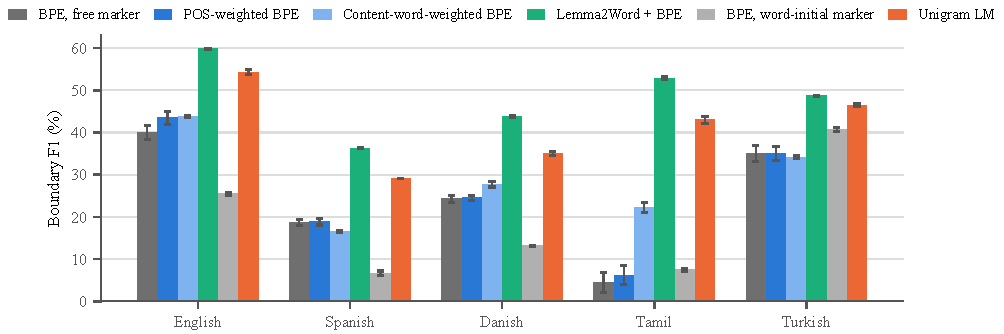
\includegraphics[width=\linewidth]{figures/fig_f1.pdf}
\caption{Boundary F1 (\%) for the six main tokenizers, over 5 languages. The bars show the average over 3 training seeds, and error bars one standard deviation.}
\label{fig:f1}
\end{figure}

The results in Table~\ref{tab:f1} also show that Lemma2Word (Section~\ref{sec:l2w}) offers the best F1 score in all languages, with a range from \nFLtwSpanish\% in Spanish to \nFLtwEnglish\% in English.
The unigram model is in second place in all languages, and leads all BPE variants by a wide margin in Tamil (F1 of \nFUniTamil{} vs.\ \nFBpeTamil).
POS-weighted BPE differs from its unweighted base by about three percentage points in English (\nFPosEnglish\% vs.\ \nFBpeEnglish\%) and by less than a point in Spanish, Danish, and Turkish.
The difference in English is the only one bigger than the variation due to random seeds.
Ablation experiments also show that the transition term alone accounts for the improvement; a version using only the transition term produces the same F1 score as the full model while a version using only the penalty term performs the same as the unweighted base model.

The F1 score using content-word weighting (Section~\ref{sec:content}) increases over plain BPE from \nFBpeTamil\% to \nFPosContentTamil\% in Tamil and by about three percentage points in English and Danish, but decreases in Spanish and Turkish.
The variant with a word-initial marker (Section~\ref{sec:freebpe}), following the SentencePiece standard, produces the worst scores in four languages because the whole word plus the marker is a single token and thus has fewer word boundaries inserted than the variant with a free marker; in Spanish for example its recall is only \nRHfBpeSpanish\% vs.\ \nRBpeSpanish\% for the free marker variant.

Figure~\ref{fig:pr} shows boundary precision versus recall for each language (points indicate the mean over the three seeds, error bars show one standard deviation, and most are smaller than the markers).

\begin{figure}[!ht]
\centering
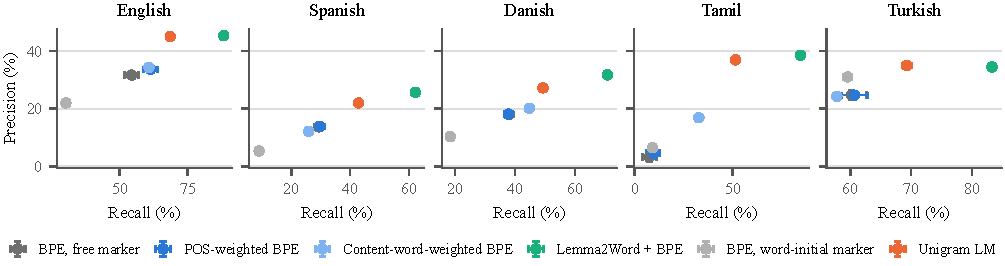
\includegraphics[width=\linewidth]{figures/fig_pr.pdf}
\caption{Boundary precision against recall per language. Points are means over three seeds and error bars span one standard deviation; most are smaller than the markers.}
\label{fig:pr}
\end{figure}

\subsection{What the Part-of-Speech Weighting Changes}\label{sec:res-pos}
The weight in Section~\ref{sec:posbpe} affects merges only at the right word boundaries, i.e.\ when a word is merged with the following space.
The effect of these merges is measured on held-out text in Table~\ref{tab:span}.
Plain free-marker BPE puts word boundaries inside tokens in \nSpanShareBpeTurkish\% to \nSpanShareBpeSpanish\% of cases (for Turkish and Spanish respectively), while the POS weighting does not change this proportion much in most languages, but reduces it from \nSpanShareBpeTamil{} to \nSpanSharePosTamil{} in Tamil\footnote{Seed 0; the three-seed mean of the share of tokens that span a boundary falls from \nCrossBpeTamil\% to \nCrossPosTamil\% (Table~\ref{tab:cross}).}.
The transitions spanned are the same ones BPE spans: in English, for example, cases of an adposition before a determiner (\texttt{of\textvisiblespace the\textvisiblespace}), in Spanish cases of determiner before noun, in Danish cases of noun before adposition.

Across all languages, variants, and with or without weighting, the mean transition probability at a spanned boundary is no more than two percentage points away from the mean over all boundaries.
The proportion of tokens crossing boundaries depends on how often each type of boundary occurs.
The transition probabilities are no more than frequencies of tag pairs and carry no additional information beyond the counts of symbols.

\begin{table}[!ht]
\centering
\caption{Percentage of word boundaries spanned by a token in held-out text, mean probability (\%) of the POS transition at spanned boundaries, and the same mean over all boundaries. Results are from seed 0; the most common spanned transition and token are shown for the POS-weighted model.}
\label{tab:span}
\footnotesize
\setlength{\tabcolsep}{3.5pt}
\begin{tabular}{llccclc}
\toprule
Language & System & spanned (\%) & $P$, spanned & $P$, all & top transition & top token \\
\midrule
English & BPE, free marker & 45.2 & 23.3 & 22.1 & ADP$\to$DET & \texttt{in\textvisiblespace{}the\textvisiblespace{}} \\
 & POS-weighted BPE & 42.6 & 23.5 & 22.1 & ADP$\to$DET & \texttt{of\textvisiblespace{}the\textvisiblespace{}} \\
 & Content-word-weighted BPE & 33.2 & 24.4 & 22.1 & ADP$\to$DET & \texttt{of\textvisiblespace{}the\textvisiblespace{}} \\
\addlinespace[2pt]
Spanish & BPE, free marker & 54.1 & 32.3 & 28.2 & DET$\to$NOUN & \texttt{a\textvisiblespace{}de\textvisiblespace{}} \\
 & POS-weighted BPE & 54.1 & 32.3 & 28.2 & DET$\to$NOUN & \texttt{a\textvisiblespace{}de\textvisiblespace{}} \\
 & Content-word-weighted BPE & 43.5 & 33.8 & 28.2 & DET$\to$NOUN & \texttt{en\textvisiblespace{}la\textvisiblespace{}} \\
\addlinespace[2pt]
Danish & BPE, free marker & 41.3 & 21.1 & 22.4 & NOUN$\to$ADP & \texttt{en\textvisiblespace{}i\textvisiblespace{}} \\
 & POS-weighted BPE & 41.4 & 21.1 & 22.4 & NOUN$\to$ADP & \texttt{en\textvisiblespace{}i\textvisiblespace{}} \\
 & Content-word-weighted BPE & 31.0 & 20.9 & 22.4 & NOUN$\to$ADP & \texttt{er\textvisiblespace{}i\textvisiblespace{}} \\
\addlinespace[2pt]
Tamil & BPE, free marker & 54.1 & 24.4 & 24.9 & NOUN$\to$NOUN & \tamil{ு}\textvisiblespace{}\tamil{ப} \\
 & POS-weighted BPE & 39.5 & 25.0 & 24.9 & NOUN$\to$NOUN & \tamil{ு}\textvisiblespace{}\tamil{ப} \\
 & Content-word-weighted BPE & 7.4 & 26.5 & 24.9 & NOUN$\to$NOUN & \tamil{ப்}\textvisiblespace{}\tamil{ப} \\
\addlinespace[2pt]
Turkish & BPE, free marker & 15.5 & 22.3 & 25.0 & NOUN$\to$CCONJ & \texttt{i\textvisiblespace{}ve\textvisiblespace{}} \\
 & POS-weighted BPE & 15.2 & 22.5 & 25.0 & NOUN$\to$CCONJ & \texttt{i\textvisiblespace{}ve\textvisiblespace{}} \\
 & Content-word-weighted BPE & 9.0 & 23.7 & 25.0 & NOUN$\to$CCONJ & \texttt{i\textvisiblespace{}ve\textvisiblespace{}} \\
\addlinespace[2pt]
\bottomrule
\end{tabular}
\end{table}


\subsection{Content-Word Weighting}\label{sec:res-content}
Doubling the weight in Section~\ref{sec:content} on merges inside some POS categories (nouns, proper nouns, verbs, adjectives) is meant to spend more of the vocabulary budget on complete content words.
That results in various benefits and drawbacks, depending on the language.
First, it decreases the percentage of cases in which a token spans a boundary in all languages (Table~\ref{tab:cross}), while in Tamil for example the recall increases from \nRBpeTamil{} to \nRPosContentTamil{} (plain BPE hardly cuts at the stem boundary).
In Spanish and Turkish however it decreases recall because whole-word tokens take the place of suffix tokens that plain BPE learns.
The weight of 2 was not tuned; varying it would make it a tuned method, which we did not do.

\subsection{Lemma2Word}\label{sec:res-l2w}
Table~\ref{tab:l2w} distinguishes between the variant that uses only learned boundaries (the lexicon variant) and the variant that lemmatizes each word on the fly using Stanza (the online variant).
All forms, forms not in training text, and UD test split forms are also reported separately.

\begin{table}[!ht]
\centering
\caption{Boundary recall and precision (\%) in Lemma2Word, by subset of words and variant. The lexicon variant uses only learned boundaries and affixes, the online variant lemmatizes the word to be tokenized with Stanza. Results averaged over three random seeds.}
\label{tab:l2w}
\small
\setlength{\tabcolsep}{3.5pt}
\begin{tabular}{llcccccc}
\toprule
 & & \multicolumn{2}{c}{all} & \multicolumn{2}{c}{unseen} & \multicolumn{2}{c}{UD test} \\
\cmidrule(lr){3-4}\cmidrule(lr){5-6}\cmidrule(lr){7-8}
Language & Variant & R & P & R & P & R & P \\
\midrule
English & lexicon & 88.2 & 45.3 & 73.7 & 30.3 & 84.0 & 37.2 \\
 & online & 98.2 & 50.9 & 98.2 & 41.1 & 91.1 & 40.9 \\
 & BPE, free marker & 54.4 & 31.6 & 54.5 & 25.5 & 49.2 & 24.8 \\
\addlinespace[2pt]
Spanish & lexicon & 62.2 & 25.6 & 40.2 & 15.3 & 48.1 & 18.3 \\
 & online & 99.1 & 39.0 & 99.1 & 35.4 & 94.8 & 34.2 \\
 & BPE, free marker & 29.4 & 13.7 & 35.8 & 14.7 & 31.8 & 13.2 \\
\addlinespace[2pt]
Danish & lexicon & 70.8 & 31.7 & 49.5 & 17.9 & 65.5 & 27.2 \\
 & online & 97.2 & 43.6 & 97.1 & 35.3 & 88.0 & 37.0 \\
 & BPE, free marker & 37.9 & 17.9 & 41.0 & 15.9 & 38.0 & 16.7 \\
\addlinespace[2pt]
Tamil & lexicon & 84.5 & 38.5 & 74.2 & 27.4 & 80.6 & 34.7 \\
 & online & 97.6 & 46.3 & 97.7 & 38.5 & 91.5 & 39.9 \\
 & BPE, free marker & 7.4 & 3.2 & 7.0 & 2.5 & 5.9 & 2.4 \\
\addlinespace[2pt]
Turkish & lexicon & 83.3 & 34.4 & 81.7 & 31.2 & 82.7 & 32.0 \\
 & online & 88.6 & 37.6 & 88.4 & 34.8 & 89.1 & 35.6 \\
 & BPE, free marker & 60.2 & 24.7 & 60.5 & 23.2 & 60.4 & 23.2 \\
\addlinespace[2pt]
\bottomrule
\end{tabular}
\end{table}


The lexicon variant has a major improvement over the unweighted BPE in recall, from \nRBpeEnglish{} to \nLtwLexiconAllREnglish{} percent in English and \nRBpeTamil{} to \nLtwLexiconAllRTamil{} percent in Tamil, and 23--34 percentage points for the other three languages.
Precision is improved as well, since BPE on the shorter pieces learns fewer internal boundaries.
The 20-occurrence threshold also admits fewer of the short and ambiguous inflectional suffixes of Spanish and Danish in combinations of word-final letter sequences.
In terms of unseen forms, recall is \nLtwLexiconUnseenREnglish{} percent in English, \nLtwLexiconUnseenRTamil{} in Tamil, and falls to a few points in Spanish and Danish for the short and ambiguous word-final letter sequences.

The online variant recovers nearly all the correct boundaries, reaching \nLtwOnlineAllRSpanish{} percent recall in Spanish because the gold boundaries were extracted from the lemmas, and the lemmatizer could recall the correct lemma from its memory on the training data.
On the UD test-split forms, which the lemmatizer never saw, recall drops, but is still within \nLtwOnlineTestRDanish--\nLtwOnlineTestRSpanish{} percent.
Its precision, however, is no better than 51 percent, because the BPE can still split inside the input pieces, while the gold standard marks only the boundaries around the word stem.

\subsection{Compression and Stability}\label{sec:res-compression}
Table~\ref{tab:tpw} reports the average tokenization efficiency, measured as the average number of tokens produced per word, on the held-out text.
The effect of the POS weighting on compression is less than one percent.
In English, Lemma2Word produces \nTpwLtwEnglish{} tokens per word compared to \nTpwBpeEnglish{} for the free-marker BPE, an increase of four percent.
In Spanish the increase is larger, eight percent, with Lemma2Word producing \nTpwLtwSpanish{} tokens per word compared to \nTpwBpeSpanish{} for the free-marker BPE.
Lemma2Word is more compact than the unigram model for all languages except Tamil.
The tokenizers that are provided as reference never cross a word boundary, and are more expensive in terms of tokens per word in the three European languages, and cheaper in the two others (Tamil, Turkish), because the free-marker BPE budget in these two languages is partly spent on tokens that cover frequent word pairs.

\begin{table}[!ht]
\centering
\caption{Tokens per whitespace word on held-out Wikipedia paragraphs (lower is more compact).}
\label{tab:tpw}
\small
\setlength{\tabcolsep}{4pt}
\begin{tabular}{lccccc}
\toprule
System & English & Spanish & Danish & Tamil & Turkish \\
\midrule
BPE, free marker & 1.481\,{\scriptsize$\pm$0.002} & 1.413\,{\scriptsize$\pm$0.002} & 1.606\,{\scriptsize$\pm$0.002} & 2.242\,{\scriptsize$\pm$0.005} & 1.962\,{\scriptsize$\pm$0.002} \\
POS-weighted BPE & 1.470\,{\scriptsize$\pm$0.001} & \textbf{1.412\,{\scriptsize$\pm$0.001}} & \textbf{1.604\,{\scriptsize$\pm$0.002}} & 2.215\,{\scriptsize$\pm$0.006} & 1.938\,{\scriptsize$\pm$0.025} \\
\quad transitions only & 1.470\,{\scriptsize$\pm$0.001} & 1.412\,{\scriptsize$\pm$0.001} & 1.604\,{\scriptsize$\pm$0.002} & 2.215\,{\scriptsize$\pm$0.006} & 1.938\,{\scriptsize$\pm$0.025} \\
\quad penalty only & \textbf{1.470\,{\scriptsize$\pm$0.001}} & 1.413\,{\scriptsize$\pm$0.002} & 1.605\,{\scriptsize$\pm$0.002} & 2.243\,{\scriptsize$\pm$0.005} & 1.962\,{\scriptsize$\pm$0.003} \\
\addlinespace[2pt]
Content-word-weighted BPE & 1.486\,{\scriptsize$\pm$0.002} & 1.423\,{\scriptsize$\pm$0.002} & 1.619\,{\scriptsize$\pm$0.001} & 2.150\,{\scriptsize$\pm$0.012} & 1.998\,{\scriptsize$\pm$0.003} \\
Lemma2Word + BPE & 1.538\,{\scriptsize$\pm$0.001} & 1.531\,{\scriptsize$\pm$0.002} & 1.703\,{\scriptsize$\pm$0.001} & 2.376\,{\scriptsize$\pm$0.002} & 2.080\,{\scriptsize$\pm$0.010} \\
BPE, word-initial marker & 1.555\,{\scriptsize$\pm$0.001} & 1.565\,{\scriptsize$\pm$0.000} & 1.713\,{\scriptsize$\pm$0.001} & \textbf{2.042\,{\scriptsize$\pm$0.001}} & \textbf{1.883\,{\scriptsize$\pm$0.002}} \\
Unigram LM & 1.609\,{\scriptsize$\pm$0.001} & 1.607\,{\scriptsize$\pm$0.002} & 1.778\,{\scriptsize$\pm$0.004} & 2.177\,{\scriptsize$\pm$0.006} & 2.004\,{\scriptsize$\pm$0.004} \\
\bottomrule
\end{tabular}
\end{table}


The reliability is measured in the appendices (Tables~\ref{tab:jaccard} and~\ref{tab:agreement}) by comparing the vocabularies produced on different training samples, and the segmentations of the same held-out text produced by different models trained on different samples using the same method.
In both cases, the reliability statistics are far less discriminative than accuracy.
The Jaccard measure of the vocabularies shows a range of 62--79 percent overlap in entries for vocabularies produced from different training samples; the segmentations produced by the same method show a range of 88--97 percent agreement.
The POS weighting does not improve these statistics, and for the overlap in the Turkish vocabulary the POS weighting is actually a detriment, going from \nJacBpeTurkish{} to \nJacPosTurkish{} percent, with a standard deviation of \nJacPosTurkishSd{} percentage points, the least stable of the cases shown in the table.
The unigram model has the lowest vocabulary overlap in all languages and the same range of agreement as all the other methods, and the difference in the vocabularies produced from the unigram model is restricted mostly to rare entries that are unlikely to be seen in the held-out text.

\subsection{Vocabulary Budget}\label{sec:res-sweep}
Comparing the performance of the different methods at two other vocabulary budgets (2,000 and 32,000 types) in Figure~\ref{fig:sweep}, the relative ranking of the methods is maintained at all budgets.
Lemma2Word improves with larger vocabularies, moving up from \nSweepFLtwEnglishVTwoK{} to \nSweepFLtwEnglishVThirtyTwoK{} percent F1 in English, for example, due to the larger budget allowing more word pieces to remain unsplit.
The unigram model moves down at 32,000 types in English, Tamil, and Turkish, where the budget exceeds what a 3,000-paragraph sample can support and whole words enter the vocabulary.
The difference between the POS-weighted BPE and the unweighted BPE is less than three percentage points at all budget sizes.

\begin{figure}[!ht]
\centering
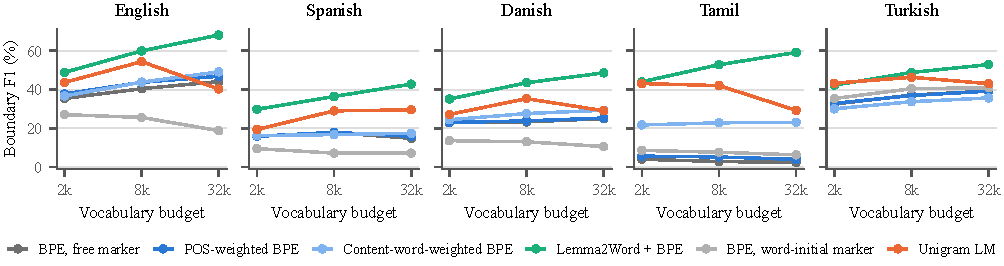
\includegraphics[width=\linewidth]{figures/fig_sweep.pdf}
\caption{Boundary F1 (\%) at vocabulary budgets of 2,000, 8,000, and 32,000 types using seed 0.}
\label{fig:sweep}
\end{figure}

\subsection{Language-Model Probe}\label{sec:res-lm}
Table~\ref{tab:bpc} reports the bits per character of the language model trained on the different tokenizers, and Figure~\ref{fig:bpc} shows the same data graphically.
A language model is trained for each tokenizer seed, and across these different seeds the standard deviation is less than 0.01 bits in most cases, and never more than 0.03 bits.
Differences of a few hundredths of a bit can therefore be considered reliable at this scale.

\begin{table}[!ht]
\centering
\caption{Bits per character in the language model trained on the output of the tokenizer. The language model has 7M parameters and is trained for 6 passes over the same text with each tokenizer. Lower scores are better, and we show the mean and one standard deviation for the three tokenizer seeds.}
\label{tab:bpc}
\small
\setlength{\tabcolsep}{4pt}
\begin{tabular}{lccccc}
\toprule
System & English & Spanish & Danish & Tamil & Turkish \\
\midrule
BPE, free marker & 2.807\,{\scriptsize$\pm$0.002} & 2.689\,{\scriptsize$\pm$0.003} & 2.878\,{\scriptsize$\pm$0.001} & 2.848\,{\scriptsize$\pm$0.006} & 2.963\,{\scriptsize$\pm$0.002} \\
POS-weighted BPE & 2.785\,{\scriptsize$\pm$0.001} & 2.687\,{\scriptsize$\pm$0.001} & 2.874\,{\scriptsize$\pm$0.001} & 2.819\,{\scriptsize$\pm$0.005} & 2.935\,{\scriptsize$\pm$0.032} \\
\quad transitions only & 2.785\,{\scriptsize$\pm$0.001} & 2.687\,{\scriptsize$\pm$0.001} & 2.874\,{\scriptsize$\pm$0.002} & 2.819\,{\scriptsize$\pm$0.005} & 2.935\,{\scriptsize$\pm$0.032} \\
\quad penalty only & 2.786\,{\scriptsize$\pm$0.002} & 2.689\,{\scriptsize$\pm$0.002} & 2.876\,{\scriptsize$\pm$0.001} & 2.849\,{\scriptsize$\pm$0.006} & 2.963\,{\scriptsize$\pm$0.003} \\
\addlinespace[2pt]
Content-word-weighted BPE & 2.794\,{\scriptsize$\pm$0.001} & 2.680\,{\scriptsize$\pm$0.003} & 2.868\,{\scriptsize$\pm$0.001} & 2.737\,{\scriptsize$\pm$0.015} & 2.995\,{\scriptsize$\pm$0.003} \\
Lemma2Word + BPE & 2.887\,{\scriptsize$\pm$0.003} & 2.861\,{\scriptsize$\pm$0.004} & 3.007\,{\scriptsize$\pm$0.001} & 2.983\,{\scriptsize$\pm$0.002} & 3.096\,{\scriptsize$\pm$0.011} \\
BPE, word-initial marker & 2.715\,{\scriptsize$\pm$0.003} & 2.674\,{\scriptsize$\pm$0.006} & 2.909\,{\scriptsize$\pm$0.003} & 2.611\,{\scriptsize$\pm$0.001} & 2.808\,{\scriptsize$\pm$0.004} \\
Unigram LM & \textbf{2.531\,{\scriptsize$\pm$0.006}} & \textbf{2.473\,{\scriptsize$\pm$0.011}} & \textbf{2.704\,{\scriptsize$\pm$0.007}} & \textbf{2.524\,{\scriptsize$\pm$0.003}} & \textbf{2.694\,{\scriptsize$\pm$0.003}} \\
\bottomrule
\end{tabular}
\end{table}


\begin{figure}[!ht]
\centering
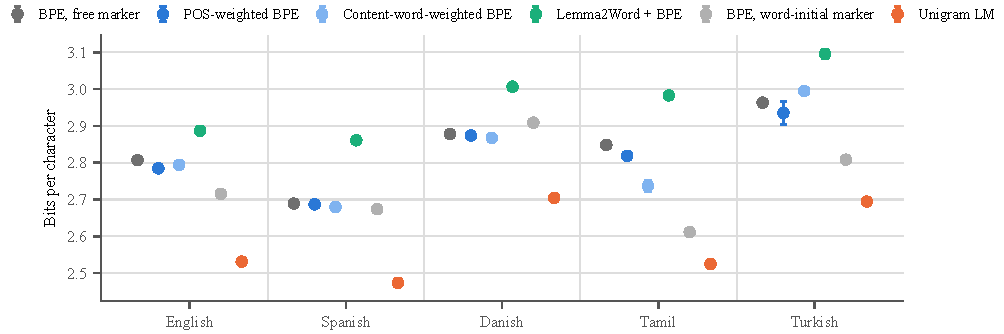
\includegraphics[width=\linewidth]{figures/fig_bpc.pdf}
\caption{Bits per character in the language model trained on the output of the tokenizer. The language model has 7M parameters and is trained for 6 passes over the same text with each tokenizer. Lower scores are better, and we show the mean and one standard deviation for the three tokenizer seeds. The y-axis starts at 2.4 bits to show the differences.}
\label{fig:bpc}
\end{figure}

However, the ordering by bits-per-character does not match the ordering by boundary-F1.
The unigram model has been ranked second by F1 and first by bits-per-character in all languages.
In English it is first with \nBpcUniEnglish{} bits-per-character compared to \nBpcBpeEnglish{} for free-marker BPE.
In Tamil the first place is taken by the unigram model with \nBpcUniTamil{} bits compared to \nBpcBpeTamil{} for free-marker BPE.
Lemma2Word has been ranked first by F1 and last by bits-per-character in all languages.
In English Lemma2Word is ranked last with \nBpcLtwEnglish{} bits-per-character.
The word cutting using stem boundaries before training the subword tokenizer is removing frequent full-word tokens and adding tokens that are too unpredictable for a model of this size to compensate.

Word-initial BPE has been ranked last by F1 in four languages.
In four languages, it has been ranked ahead of free-marker BPE by bits-per-character.
In English it is ranked ahead with \nBpcHfBpeEnglish{} vs.\ \nBpcBpeEnglish.
The tokens crossing word boundaries, which help compactness in free-marker BPE, do not help in prediction.
POS weighting has been changing bits-per-character by less than 0.03 in all the languages, so it seems it is pointing in a positive direction but with a small contribution.
Interestingly, the table shows that for Turkish the seed-to-seed variation in bits-per-character is the highest.
The two ablations with POS weighting give the same result.
Content word weighting has been reducing bits-per-character in Tamil to \nBpcPosContentTamil{} vs.\ \nBpcBpeTamil.
This was also the language where it has been giving the largest improvement in boundary-F1.
On the other hand, in Turkish content-word weighting has been increasing the bits-per-character numbers.

Since all the tokenizers are trained on the same text, the number of passes is the same for all models; they go over the data 6 times.
Since a higher token count therefore leads to more optimizer steps, the unigram model has 8.6\% more optimizer steps than free-marker BPE in English.
To control for the change in optimizer steps, we have trained a model for free-marker BPE in seed 0 with 10\% fewer optimizer steps (5.4 passes over the data) and 10\% more optimizer steps (6.6 passes).
The bits-per-character changes from \nBpcControlBase{} to \nBpcControlLow{} and \nBpcControlHigh{} respectively.
These changes are small compared to the ones between tokenizers, so the step count cannot be used to explain the model ranking.
Since Lemma2Word has a higher number of tokens than free-marker BPE and it has been ranked behind, the reason cannot be the optimizer step count alone.

These results indicate that morphological alignment and the quality of the model do not move together at this scale, which agrees with the conclusions reached about the unigram model by \citet{bostrom2020bpe}.
This also supports the finding that the intrinsic measures for tokenizers are not perfect predictors for downstream tasks~\cite{ali2024tokenizer,schmidt2024tokenization}.

\subsection{A Language Model as a Segmenter}\label{sec:res-llm}
Table~\ref{tab:llm} shows the results of the study described in Section~\ref{sec:llm}.
For each language, a sample of 400 word forms were randomly selected from the gold standard list using seed 0.
The Claude Sonnet model (\texttt{claude-sonnet-5-5}, October 2026 version) was selected and it was prompted to add plus signs between morphemes in batches of 40 words.
The prompt used does not allow any character modification and is given in Appendix~\ref{app:prompt}.
Answers that change the characters of the word are invalid and they were not counted when computing the scores.
To compare with the same seed 0 tokenizers, we have evaluated them on the same words that the model had given valid answers for.

\begin{table}[!ht]
\centering
\caption{Claude Sonnet segmenting words into morphemes, on a fixed random sample of gold standard forms. The seed 0 tokenizers are evaluated on the same words. Invalid answers are answers that change the characters of the word and they were not counted in the computation of the scores. The table reports boundary precision, recall and F1 (in \%), and the number of tokens per word after segmentation.}
\label{tab:llm}
\small
\setlength{\tabcolsep}{3.5pt}
\begin{tabular}{lrrcccccccc}
\toprule
 & & & \multicolumn{4}{c}{language model} & \multicolumn{3}{c}{recall of tokenizers on the same words} \\
\cmidrule(lr){4-7}\cmidrule(lr){8-10}
Language & words & invalid & P & R & F1 & pieces/word & Lemma2Word & Unigram & BPE, free \\
\midrule
English & 400 & 0 & 77.6 & 91.0 & 83.8 & 2.17 & 87.0 & 69.2 & 52.2 \\
Spanish & 399 & 1 & 35.1 & 69.9 & 46.8 & 2.99 & 62.2 & 44.1 & 25.3 \\
Danish & 400 & 0 & 38.9 & 66.0 & 49.0 & 2.69 & 72.5 & 50.0 & 42.0 \\
Tamil & 393 & 7 & 72.6 & 90.4 & 80.5 & 2.25 & 84.8 & 48.9 & 6.8 \\
Turkish & 400 & 0 & 50.7 & 96.5 & 66.5 & 2.90 & 84.8 & 67.2 & 60.2 \\
\bottomrule
\end{tabular}
\end{table}


The model has been able to surpass the recall on gold boundaries of any of the tokenizers in four languages.
In English the model gets \nLlmREnglish\% compared to \nLlmSampleLtwREnglish\% for Lemma2Word, in Tamil \nLlmRTamil\% vs.\ \nLlmSampleLtwRTamil\% and in Turkish \nLlmRTurkish\% vs.\ \nLlmSampleLtwRTurkish\%.
The model has been ranked behind Lemma2Word in Danish with \nLlmRDanish\% recall vs.\ \nLlmSampleLtwRDanish\%.
The precision of the model is ranging between \nLlmPSpanish\% and \nLlmPEnglish\%.
The model marks derivational affixes and parts of compounds that are not included in the lemma-based gold standard, and the number of pieces per word is between \nLlmTpwEnglish{} and \nLlmTpwSpanish{} compared to the maximum of 3 pieces per word in the gold.
Almost all of the answers preserve the characters of the words in the Latin script, and there was only \nLlmInvalidSpanish{} invalid answer for Spanish and none for the other Latin-script languages.

Tamil had two issues.
The model had long reasoning chains, the 40-word batches exceeded the response length, and the unanswered words had to be re-asked in 15-word batches.
The model had also written the underlying morphemes in \nLlmInvalidTamil{} answers rather than the surface forms, violating the character constraint.
In one of them the model gave \tamil{கள்}\,+\,\tamil{உக்கு} instead of \tamil{களுக்கு}, since the suffix vowel fuses with the consonant.
The study used approximately 2,000 words and the cost of the API was minimal (a few dollars).
This evaluation is not showing what a tokenizer built on top of the model's responses would be capable of, but what the model knows about the morphology.
The answers from the model do not have a fixed vocabulary and they are not guaranteed to be in a consistent format even if the same word occurs multiple times.
The cost per word is several orders of magnitude more than any of the tokenizers shown in Table~\ref{tab:f1}.
The answers could be used off-line to generate a segmentation lexicon similar to the output of Lemma2Word to provide boundaries in places where a lemmatizer doesn't exist.
This use case is not evaluated in the paper.


\section{Discussion}\label{sec:discussion}

The transition-weighting fails because it adds no new signal.
The basic BPE merge score is just the count of a pair of adjacent symbols.
The variant that uses POS weighting simply multiplies this count by one plus the probability of the corresponding transition in the tag sequence, when the pair of symbols is spanning the boundary between two words.
This is a smoothing of the original symbol-pair count, because the transition probability is simply a function of the pair of tags and the tags are functions of the words.
In the case of the pair \emph{of the}, the high frequency results in a merge, and the weighting just adds incentive towards this frequent pair.

As Table~\ref{tab:span} shows, the same tokens bridge the word boundary with and without weighting.
There is no signal pointing to the right place to split at a token boundary, since the probability of a transition at a boundary spanned by a token is never greater than the probability of a transition at an unspanned boundary.
The design simply never intended to signal the right place to split, which is what is needed to find the gold boundaries in the middle of words.

In the preliminary results reported earlier, the segmentation entropy was lower in the tokenization using POS tagging, the tokens were longer, the transition accuracy diagnostic showed gains of 12--20 points, and vocabulary reuse showed gains of about 20 points.
These were not measured on held-out words, or against a gold standard.
The implementation used was the same as that with the bug in Section~\ref{sec:posbpe} of comparing the transitions against the wrong words after the first space-absorbing merge.
Under the protocol in Section~\ref{sec:protocol}, there was no change in vocabulary reuse (Table~\ref{tab:jaccard}), and less than 1\% change in the length of the tokens (Table~\ref{tab:tpw}).
And the only method that consistently improved the detection of morphological boundaries is the one using a lemmatizer.

The lemma carries information about the end of the stem, whereas the tag classifies the type of word, and only the lemma contributes information about the boundary.
The Lemma2Word method has 23 to 77 point gains in recall, of which the proportion generalizing to out-of-vocabulary words depends on the generalization in the inventories of the affixes.
This is good in English and Turkish, where the suffixes are long and distinct, and bad in Spanish and Danish, where the suffixes are short.
The online version generalizes through the lemmatizer and reaches 88\%--95\% recall on the forms in the treebank test set, but requires a neural lemmatizer to run online during the tokenization and uses the same training data as the gold standard.

The content-word weighting sits between the two.
It uses the tags to make the boundary decision by choosing the words that are preserved as whole words.
It helps in the case where the budget was missing whole words, as in the case of content words in Tamil, but hurts in the case where the budget could be better spent on suffixes, as in Spanish and Turkish.

The probe in Section~\ref{sec:res-lm} separates two things that the literature on morphology-aware tokenization often conflates.
The probe shows that more gold boundaries does not mean better downstream performance for the language model.
The tokenizer that finds the most boundaries, Lemma2Word, is the one that corresponds to the worst model performance.
The unigram model, which finds fewer boundaries but segments text according to a probabilistic model, is the one that corresponds to the best performance, by about a quarter of a bit per character.
The probe is small in scale, and a larger model using more text may change or invert these differences.
However, this direction is consistent with \citet{bostrom2020bpe}, who found that unigram segmentation performs at least as well as BPE in pretraining, and the results by \citet{ali2024tokenizer} and \citet{schmidt2024tokenization}, who find that performance on intrinsic measures of tokenizers is poorly predictive of performance on downstream tasks.
The importance of the result is that a score on the morphological boundaries is not in itself a sufficient justification to use a tokenizer.

The space marker convention is another factor that is rarely considered.
The original implementation is such that the space marker is freely merged.
In this implementation, 4\%--22\% of the tokens span a word boundary.
This increases the boundary F1 over the word-initial marker convention in four languages.
This is because the whole words with a space marker prefixed are not single tokens.
This means that the budget of whole words is spent on smaller pieces.
This however disagrees with the probe, which finds a preference for the word-initial marker convention in the same four languages.
This is as important as the linguistic signals chosen.
The comparisons between different tokenizers should maintain a fixed convention for the space marker.

There are limitations in this study.
The gold standard is limited to two boundaries per word, which are around the stem.
This means that the internal structure of the derivational morphology is counted against precision.
This makes recall the more reliable metric, although the ordering of the methods is unchanged.
The training samples are small with 3,000 paragraphs from each language.
This is in part because the implementation is pure Python for the free space marker convention.
The sweeps in vocabulary size show that the order of the methods is the same at each budget, but the absolute numbers can change in larger corpora.
The tags and lemmas are from the same tagger.
The Tamil treebank is the smallest of the five treebanks used.
The language model probe uses a small model with 7M parameters that was trained for minutes only.
This is able to show tokenizer differences at the scale of this probe, but not at the scale of a large language model.

\section{Conclusion}\label{sec:conclusion}
Using part-of-speech (POS) and lemma information in subword tokenizers in five languages, we assess them under one protocol: gold morpheme boundaries, held-out text, repeated training samples and a language model probe.
Weighting subword merges by POS transitions does not change token boundaries or output, because the transition probability only describes the order of words, not internal word structure.
Weighting subword merges within content words changes the vocabulary as desired, but does not always give a better accuracy than without.

Using lemmas to deduce word boundaries instead increases boundary recall by 23 to 77 points, at the cost of 4--8\% more tokens.
How much of the gain carries over to unseen words depends on the distinctiveness of a language's affixes.
If a tokenizer is to include morphological boundaries, it should use a lemmatizer or segmentation lexicon, where a tagger does not provide any value.
However, the quality of these boundaries for language models is a question in itself.
A language model probe ranks these tokenizers differently than the boundary scores, with the unigram model first and Lemma2Word last in each language, and will need larger scale than our 7M-parameter language model to resolve.
Morphological alignment cannot yet be recommended as a goal.


{\sloppy
\paragraph{Author contributions.}
% DRAFT -- all authors must agree on this text before posting.
A.C., J.D.\ and M.V.\ designed the POS-weighted tokenizer, Lemma2Word and the language model segmentation study and wrote the original report.
J.D.\ re-implemented, corrected and evaluated the tokenizers, ran the experiments and wrote the current report.
% TODO: describe each author's part of the original implementation.

\par}

\bibliographystyle{plainnat}
\bibliography{refs}

\appendix
\section{Precision, Recall and Stability by Language}\label{app:tables}
\begin{table}[!ht]
\centering
\caption{Boundary precision (\%).}
\label{tab:precision}
\small
\setlength{\tabcolsep}{4pt}
\begin{tabular}{lccccc}
\toprule
System & English & Spanish & Danish & Tamil & Turkish \\
\midrule
BPE, free marker & 31.6\,{\scriptsize$\pm$1.2} & 13.7\,{\scriptsize$\pm$0.5} & 17.9\,{\scriptsize$\pm$0.6} & 3.2\,{\scriptsize$\pm$1.7} & 24.7\,{\scriptsize$\pm$1.4} \\
POS-weighted BPE & 33.6\,{\scriptsize$\pm$1.1} & 13.8\,{\scriptsize$\pm$0.6} & 18.1\,{\scriptsize$\pm$0.3} & 4.5\,{\scriptsize$\pm$1.7} & 24.6\,{\scriptsize$\pm$1.3} \\
\quad transitions only & 33.6\,{\scriptsize$\pm$1.2} & 13.8\,{\scriptsize$\pm$0.6} & 18.1\,{\scriptsize$\pm$0.3} & 4.6\,{\scriptsize$\pm$1.7} & 24.6\,{\scriptsize$\pm$1.3} \\
\quad penalty only & 32.7\,{\scriptsize$\pm$0.9} & 13.7\,{\scriptsize$\pm$0.5} & 18.0\,{\scriptsize$\pm$0.7} & 3.2\,{\scriptsize$\pm$1.7} & 24.6\,{\scriptsize$\pm$1.5} \\
\addlinespace[2pt]
Content-word-weighted BPE & 34.3\,{\scriptsize$\pm$0.2} & 12.1\,{\scriptsize$\pm$0.2} & 20.1\,{\scriptsize$\pm$0.5} & 16.8\,{\scriptsize$\pm$0.9} & 24.2\,{\scriptsize$\pm$0.3} \\
Lemma2Word + BPE & \textbf{45.3\,{\scriptsize$\pm$0.1}} & \textbf{25.6\,{\scriptsize$\pm$0.1}} & \textbf{31.7\,{\scriptsize$\pm$0.2}} & \textbf{38.5\,{\scriptsize$\pm$0.4}} & 34.4\,{\scriptsize$\pm$0.1} \\
BPE, word-initial marker & 22.0\,{\scriptsize$\pm$0.3} & 5.3\,{\scriptsize$\pm$0.4} & 10.2\,{\scriptsize$\pm$0.1} & 6.4\,{\scriptsize$\pm$0.3} & 31.0\,{\scriptsize$\pm$0.3} \\
Unigram LM & 45.0\,{\scriptsize$\pm$0.5} & 21.9\,{\scriptsize$\pm$0.0} & 27.2\,{\scriptsize$\pm$0.4} & 36.9\,{\scriptsize$\pm$0.8} & \textbf{35.0\,{\scriptsize$\pm$0.3}} \\
\bottomrule
\end{tabular}
\end{table}

\begin{table}[!ht]
\centering
\caption{Boundary recall (\%).}
\label{tab:recall}
\small
\setlength{\tabcolsep}{4pt}
\begin{tabular}{lccccc}
\toprule
System & English & Spanish & Danish & Tamil & Turkish \\
\midrule
BPE, free marker & 54.4\,{\scriptsize$\pm$2.6} & 29.4\,{\scriptsize$\pm$1.5} & 37.9\,{\scriptsize$\pm$1.5} & 7.4\,{\scriptsize$\pm$3.7} & 60.2\,{\scriptsize$\pm$2.4} \\
POS-weighted BPE & 61.3\,{\scriptsize$\pm$2.5} & 29.8\,{\scriptsize$\pm$1.5} & 37.9\,{\scriptsize$\pm$1.3} & 9.5\,{\scriptsize$\pm$3.3} & 60.7\,{\scriptsize$\pm$2.1} \\
\quad transitions only & 61.3\,{\scriptsize$\pm$2.5} & 29.8\,{\scriptsize$\pm$1.5} & 37.9\,{\scriptsize$\pm$1.3} & 9.6\,{\scriptsize$\pm$3.3} & 60.7\,{\scriptsize$\pm$2.1} \\
\quad penalty only & 58.7\,{\scriptsize$\pm$2.0} & 29.4\,{\scriptsize$\pm$1.5} & 37.9\,{\scriptsize$\pm$1.6} & 7.4\,{\scriptsize$\pm$3.7} & 60.1\,{\scriptsize$\pm$2.5} \\
\addlinespace[2pt]
Content-word-weighted BPE & 60.8\,{\scriptsize$\pm$0.3} & 25.9\,{\scriptsize$\pm$0.5} & 44.8\,{\scriptsize$\pm$1.1} & 32.7\,{\scriptsize$\pm$1.6} & 57.8\,{\scriptsize$\pm$0.4} \\
Lemma2Word + BPE & \textbf{88.2\,{\scriptsize$\pm$0.1}} & \textbf{62.2\,{\scriptsize$\pm$0.3}} & \textbf{70.8\,{\scriptsize$\pm$0.5}} & \textbf{84.5\,{\scriptsize$\pm$0.5}} & \textbf{83.3\,{\scriptsize$\pm$0.3}} \\
BPE, word-initial marker & 30.3\,{\scriptsize$\pm$0.4} & 9.1\,{\scriptsize$\pm$0.7} & 18.4\,{\scriptsize$\pm$0.2} & 9.0\,{\scriptsize$\pm$0.4} & 59.6\,{\scriptsize$\pm$0.7} \\
Unigram LM & 68.6\,{\scriptsize$\pm$0.4} & 42.9\,{\scriptsize$\pm$0.2} & 49.3\,{\scriptsize$\pm$0.6} & 51.5\,{\scriptsize$\pm$0.9} & 69.3\,{\scriptsize$\pm$0.7} \\
\bottomrule
\end{tabular}
\end{table}

\begin{table}[!ht]
\centering
\caption{Share of held-out tokens that span a word boundary (\%).}
\label{tab:cross}
\small
\setlength{\tabcolsep}{4pt}
\begin{tabular}{lccccc}
\toprule
System & English & Spanish & Danish & Tamil & Turkish \\
\midrule
BPE, free marker & 15.2\,{\scriptsize$\pm$0.1} & 18.3\,{\scriptsize$\pm$0.0} & 13.1\,{\scriptsize$\pm$0.1} & \textbf{22.0\,{\scriptsize$\pm$1.5}} & 4.5\,{\scriptsize$\pm$0.1} \\
POS-weighted BPE & 14.2\,{\scriptsize$\pm$0.1} & 18.4\,{\scriptsize$\pm$0.0} & 13.2\,{\scriptsize$\pm$0.2} & 15.6\,{\scriptsize$\pm$2.4} & 4.4\,{\scriptsize$\pm$0.1} \\
\quad transitions only & 14.2\,{\scriptsize$\pm$0.1} & 18.4\,{\scriptsize$\pm$0.0} & 13.2\,{\scriptsize$\pm$0.2} & 15.6\,{\scriptsize$\pm$2.4} & 4.4\,{\scriptsize$\pm$0.1} \\
\quad penalty only & 14.4\,{\scriptsize$\pm$0.0} & 18.3\,{\scriptsize$\pm$0.0} & 13.2\,{\scriptsize$\pm$0.1} & 21.9\,{\scriptsize$\pm$1.5} & 4.5\,{\scriptsize$\pm$0.1} \\
\addlinespace[2pt]
Content-word-weighted BPE & 10.9\,{\scriptsize$\pm$0.2} & 14.5\,{\scriptsize$\pm$0.1} & 9.7\,{\scriptsize$\pm$0.2} & 2.2\,{\scriptsize$\pm$0.3} & 2.5\,{\scriptsize$\pm$0.1} \\
Lemma2Word + BPE & \textbf{15.7\,{\scriptsize$\pm$0.0}} & \textbf{19.2\,{\scriptsize$\pm$0.0}} & \textbf{15.4\,{\scriptsize$\pm$0.1}} & 12.8\,{\scriptsize$\pm$0.2} & \textbf{6.6\,{\scriptsize$\pm$0.1}} \\
BPE, word-initial marker & 0.0\,{\scriptsize$\pm$0.0} & 0.0\,{\scriptsize$\pm$0.0} & 0.0\,{\scriptsize$\pm$0.0} & 0.0\,{\scriptsize$\pm$0.0} & 0.0\,{\scriptsize$\pm$0.0} \\
Unigram LM & 0.0\,{\scriptsize$\pm$0.0} & 0.0\,{\scriptsize$\pm$0.0} & 0.0\,{\scriptsize$\pm$0.0} & 0.0\,{\scriptsize$\pm$0.0} & 0.0\,{\scriptsize$\pm$0.0} \\
\bottomrule
\end{tabular}
\end{table}

\begin{table}[!ht]
\centering
\caption{Vocabulary reuse: Jaccard overlap (\%) between the vocabularies learned from different training samples (three seed pairs).}
\label{tab:jaccard}
\small
\setlength{\tabcolsep}{4pt}
\begin{tabular}{lccccc}
\toprule
System & English & Spanish & Danish & Tamil & Turkish \\
\midrule
BPE, free marker & 76.8\,{\scriptsize$\pm$0.8} & 75.8\,{\scriptsize$\pm$1.8} & 76.8\,{\scriptsize$\pm$0.4} & 63.8\,{\scriptsize$\pm$4.8} & 74.6\,{\scriptsize$\pm$1.9} \\
POS-weighted BPE & 77.8\,{\scriptsize$\pm$0.9} & 76.3\,{\scriptsize$\pm$2.0} & 76.7\,{\scriptsize$\pm$0.6} & 61.9\,{\scriptsize$\pm$5.4} & 67.1\,{\scriptsize$\pm$7.4} \\
\quad transitions only & 77.8\,{\scriptsize$\pm$0.9} & 76.2\,{\scriptsize$\pm$2.0} & 76.6\,{\scriptsize$\pm$0.5} & 61.8\,{\scriptsize$\pm$5.4} & 67.2\,{\scriptsize$\pm$7.4} \\
\quad penalty only & 77.1\,{\scriptsize$\pm$0.7} & 75.8\,{\scriptsize$\pm$1.8} & 76.3\,{\scriptsize$\pm$0.4} & 64.1\,{\scriptsize$\pm$4.8} & 75.1\,{\scriptsize$\pm$2.3} \\
\addlinespace[2pt]
Content-word-weighted BPE & 74.8\,{\scriptsize$\pm$3.1} & \textbf{77.2\,{\scriptsize$\pm$0.3}} & 74.3\,{\scriptsize$\pm$2.4} & 71.5\,{\scriptsize$\pm$2.5} & 77.0\,{\scriptsize$\pm$1.0} \\
Lemma2Word + BPE & 76.9\,{\scriptsize$\pm$0.7} & 75.6\,{\scriptsize$\pm$1.5} & \textbf{77.8\,{\scriptsize$\pm$0.6}} & 74.8\,{\scriptsize$\pm$0.5} & 74.1\,{\scriptsize$\pm$3.1} \\
BPE, word-initial marker & \textbf{78.5\,{\scriptsize$\pm$0.4}} & 74.4\,{\scriptsize$\pm$3.2} & 76.1\,{\scriptsize$\pm$0.9} & \textbf{76.9\,{\scriptsize$\pm$0.2}} & \textbf{78.5\,{\scriptsize$\pm$1.1}} \\
Unigram LM & 69.3\,{\scriptsize$\pm$1.1} & 66.3\,{\scriptsize$\pm$0.7} & 62.7\,{\scriptsize$\pm$0.2} & 62.9\,{\scriptsize$\pm$0.6} & 69.1\,{\scriptsize$\pm$0.4} \\
\bottomrule
\end{tabular}
\end{table}

\begin{table}[!ht]
\centering
\caption{Segmentation agreement: boundary F1 (\%) between the held-out segmentations of tokenizers trained on different samples (three seed pairs).}
\label{tab:agreement}
\small
\setlength{\tabcolsep}{4pt}
\begin{tabular}{lccccc}
\toprule
System & English & Spanish & Danish & Tamil & Turkish \\
\midrule
BPE, free marker & 95.2\,{\scriptsize$\pm$0.1} & 95.1\,{\scriptsize$\pm$0.8} & 95.7\,{\scriptsize$\pm$0.2} & 88.6\,{\scriptsize$\pm$3.4} & 94.6\,{\scriptsize$\pm$1.2} \\
POS-weighted BPE & 95.8\,{\scriptsize$\pm$0.1} & 95.2\,{\scriptsize$\pm$0.9} & 95.5\,{\scriptsize$\pm$0.3} & 87.5\,{\scriptsize$\pm$3.3} & 92.5\,{\scriptsize$\pm$2.7} \\
\quad transitions only & 95.8\,{\scriptsize$\pm$0.1} & 95.3\,{\scriptsize$\pm$0.9} & 95.5\,{\scriptsize$\pm$0.3} & 87.6\,{\scriptsize$\pm$3.4} & 92.5\,{\scriptsize$\pm$2.7} \\
\quad penalty only & 95.6\,{\scriptsize$\pm$0.2} & 95.1\,{\scriptsize$\pm$0.8} & 95.5\,{\scriptsize$\pm$0.1} & 88.7\,{\scriptsize$\pm$3.5} & 94.7\,{\scriptsize$\pm$1.3} \\
\addlinespace[2pt]
Content-word-weighted BPE & 95.0\,{\scriptsize$\pm$1.1} & \textbf{95.9\,{\scriptsize$\pm$0.1}} & 95.5\,{\scriptsize$\pm$0.6} & 94.0\,{\scriptsize$\pm$0.9} & \textbf{96.0\,{\scriptsize$\pm$0.2}} \\
Lemma2Word + BPE & 95.2\,{\scriptsize$\pm$0.3} & 94.9\,{\scriptsize$\pm$0.6} & 95.8\,{\scriptsize$\pm$0.2} & 94.7\,{\scriptsize$\pm$0.2} & 95.6\,{\scriptsize$\pm$0.7} \\
BPE, word-initial marker & \textbf{96.9\,{\scriptsize$\pm$0.1}} & 95.5\,{\scriptsize$\pm$1.2} & \textbf{95.9\,{\scriptsize$\pm$0.1}} & \textbf{95.4\,{\scriptsize$\pm$0.2}} & 95.8\,{\scriptsize$\pm$0.6} \\
Unigram LM & 95.0\,{\scriptsize$\pm$0.1} & 94.1\,{\scriptsize$\pm$0.2} & 93.5\,{\scriptsize$\pm$0.2} & 93.5\,{\scriptsize$\pm$0.1} & 94.3\,{\scriptsize$\pm$0.2} \\
\bottomrule
\end{tabular}
\end{table}


\section{Example Segmentations}\label{app:examples}
\begin{table}[!ht]
\centering
\caption{Example segmentations of evaluation words absent from the training text (seed 0). The evaluation words are taken from unseen forms without capitals, have between 8 and 14 characters and at least one gold boundary. We show the first, middle and last word of an alphabetically sorted list. To save space, the word-initial-marker BPE is omitted. Vertical bars (|) indicate boundaries, and gold contains the ground-truth boundaries inferred from the lemma.}
\label{tab:examples}
\scriptsize
\setlength{\tabcolsep}{2.5pt}
\begin{tabular}{llllll}
\toprule
Lang. & Gold & BPE, free marker & Content-weighted & Lemma2Word & Unigram \\
\midrule
En & \texttt{abduct|ed} & \texttt{ab|duct|ed} & \texttt{ab|duct|ed} & \texttt{ab|duc|t|ed} & \texttt{a|b|du|c|ted} \\
En & \texttt{interrupt|ing} & \texttt{inter|rupt|ing} & \texttt{inter|rupt|ing} & \texttt{inter|rup|t|ing} & \texttt{interrupt|ing} \\
En & \texttt{youngster|s} & \texttt{young|st|ers} & \texttt{young|st|ers} & \texttt{young|ster|s} & \texttt{young|ster|s} \\
\addlinespace[2pt]
Sp & \texttt{abandonado|s} & \texttt{abandon|ados} & \texttt{abandon|ados} & \texttt{abandon|a|dos} & \texttt{abandonado|s} \\
Sp & \texttt{galeote|s} & \texttt{gal|e|ot|es} & \texttt{gal|e|ot|es} & \texttt{gal|e|ot|es} & \texttt{gal|eo|tes} \\
Sp & \texttt{ímprobo|s} & \texttt{í|m|prob|os} & \texttt{í|m|prob|os} & \texttt{í|m|prob|os} & \texttt{í|mp|ro|bo|s} \\
\addlinespace[2pt]
Da & \texttt{abonnent|erne} & \texttt{ab|on|n|ent|erne} & \texttt{abon|n|ent|ern|e} & \texttt{ab|on|n|ent|erne} & \texttt{ab|on|n|en|t|erne} \\
Da & \texttt{landshold|ets} & \texttt{lands|hol|det|s} & \texttt{lands|hold|et|s} & \texttt{lands|hold|et|s} & \texttt{lands|hold|ets} \\
Da & \texttt{østmagt|ernes} & \texttt{øst|magt|ern|es} & \texttt{øst|magt|ern|es} & \texttt{øst|magt|erne|s} & \texttt{øst|magt|ernes} \\
\addlinespace[2pt]
Ta & \tamil{gஎர்மனி|யில்} & \tamil{g|எ|ர்மன|ிய|ில்} & \tamil{g|எ|ர்மன|ிய|ில்} & \tamil{g|எ|ர்ம|னி|யில்} & \tamil{g|எ|ர்|ம|னி|யில்} \\
Ta & \tamil{தற்கொலை|ப்} & \tamil{தற்க|ொலைப|்} & \tamil{தற்கொ|லை|ப்} & \tamil{தற்க|ொ|ல|ை|ப்} & \tamil{தற்கொலை|ப்} \\
Ta & \tamil{ஹென்றி|யின்} & \tamil{ஹ|ென்ற|ிய|ின்} & \tamil{ஹெ|ன்ற|ிய|ின்} & \tamil{ஹெ|ன்ற|ி|ய|ின்} & \tamil{ஹென்றி|யின்} \\
\addlinespace[2pt]
Tu & \texttt{abajur|lara} & \texttt{ab|aj|ur|lar|a} & \texttt{ab|aj|ur|lar|a} & \texttt{aba|j|ur|lar|a} & \texttt{a|ba|j|ur|lara} \\
Tu & \texttt{korkala|mıştı} & \texttt{kor|kal|amış|tı} & \texttt{kor|kal|amış|t|ı} & \texttt{kor|kal|amış|tı} & \texttt{kor|ka|la|mıştı} \\
Tu & \texttt{şıpıdık|larının} & \texttt{ş|ıp|ı|dık|ların|ın} & \texttt{ş|ıp|ıd|ık|larının} & \texttt{ş|ıp|ı|dık|ların|ın} & \texttt{ş|ıp|ı|dıkları|nın} \\
\addlinespace[2pt]
\bottomrule
\end{tabular}
\end{table}


\section{Prompt of the Segmentation Study}\label{app:prompt}
The language model was prompted with the following text string, which contained the name of the respective language and a batch of words, one per line.
\begin{quote}\small\ttfamily\raggedright
Segment each \{lang\} word below into its morphemes: prefixes, the stem, and suffixes (inflectional and derivational).\\
Rules: keep every character of the word exactly as given and in order; insert a plus sign ({+}) at each morpheme boundary; a word with a single morpheme is returned unchanged; do not add explanations.\\
Answer with one line per word in the format \ \ word: seg{+}men{+}ted \ \ and nothing else.\par\medskip
\{words\}
\end{quote}

\section{Reproduction}\label{app:repro}
The repository contains all the code and data preparation scripts, as well as the metrics for each run.
We present the commands here to reproduce all the numbers, tables and figures.
\begin{enumerate}
\item \texttt{python experiments/fetch\_corpus.py} fetches the corpus from Wikipedia paragraphs.
\item \texttt{bash experiments/tag\_all.sh} runs the tagging and lemma tasks using Stanza.
\item \texttt{bash experiments/run\_all.sh} runs the main experiments, over five languages, eight methods, and three seeds.
\item \texttt{bash experiments/run\_sweep.sh} runs the sweep experiments with two type counts (2,000 and 32,000) and seed 0.
\item \texttt{bash experiments/after\_grid.sh} runs the language model probes.
\item \texttt{python experiments/llm\_segment.py} runs the large language model segmentation study.
\item \texttt{python experiments/aggregate.py} produces \texttt{numbers.tex}, tables, and figures.
\end{enumerate}
Gold boundaries come from the Hugging Face dataset \path{catherinearnett/morphscore}, and text from the Hugging Face dataset \path{wikimedia/wikipedia}.

\end{document}
